%%% Hlavní soubor. Zde se definují základní parametry a odkazuje se na ostatní části. %%%

%% Verze pro jednostranný tisk:
% Okraje: levý 40mm, pravý 25mm, horní a dolní 25mm
% (ale pozor, LaTeX si sám přidává 1in)
\documentclass[12pt,a4paper]{report}
\setlength\textwidth{145mm}
\setlength\textheight{247mm}
\setlength\oddsidemargin{15mm}
\setlength\evensidemargin{15mm}
\setlength\topmargin{0mm}
\setlength\headsep{0mm}
\setlength\headheight{0mm}
% \openright zařídí, aby následující text začínal na pravé straně knihy
\let\openright=\clearpage

%% Pokud tiskneme oboustranně:
% \documentclass[12pt,a4paper,twoside,openright]{report}
% \setlength\textwidth{145mm}
% \setlength\textheight{247mm}
% \setlength\oddsidemargin{14.2mm}
% \setlength\evensidemargin{0mm}
% \setlength\topmargin{0mm}
% \setlength\headsep{0mm}
% \setlength\headheight{0mm}
% \let\openright=\cleardoublepage

\usepackage[usenames]{xcolor}  % barevná sazba

%% Vytváříme PDF/A-2u
\usepackage[a-2u]{pdfx}

%% Přepneme na českou sazbu a fonty Latin Modern
\usepackage[slovak]{babel}
\usepackage{lmodern}
\usepackage[T1]{fontenc}
\usepackage{textcomp}

%% Použité kódování znaků: obvykle latin2, cp1250 nebo utf8:
\usepackage[utf8]{inputenc}

%%% Další užitečné balíčky (jsou součástí běžných distribucí LaTeXu)
\usepackage{amsmath}        % rozšíření pro sazbu matematiky
\usepackage{amsfonts}       % matematické fonty
\usepackage{amsthm}         % sazba vět, definic apod.
\usepackage{bbding}         % balíček s nejrůznějšími symboly
			    % (čtverečky, hvězdičky, tužtičky, nůžtičky, ...)
\usepackage{bm}             % tučné symboly (příkaz \bm)
\usepackage{graphicx}       % vkládání obrázků
\usepackage{fancyvrb}       % vylepšené prostředí pro strojové písmo
\usepackage{indentfirst}    % zavede odsazení 1. odstavce kapitoly
\usepackage{natbib}         % zajištuje možnost odkazovat na literaturu
			    % stylem AUTOR (ROK), resp. AUTOR [ČÍSLO]
\usepackage[nottoc]{tocbibind} % zajistí přidání seznamu literatury,
                            % obrázků a tabulek do obsahu
\usepackage{icomma}         % inteligetní čárka v matematickém módu+\usepackage{dcolumn}        % lepší zarovnání sloupců v tabulkách
\usepackage{booktabs}       % lepší vodorovné linky v tabulkách
\usepackage{paralist}       % lepší enumerate a itemize


\usepackage{listings}
\usepackage{color}

\usepackage{multicol}
\usepackage{multirow}

%%% Údaje o práci

% Název práce v jazyce práce (přesně podle zadání)
\def\NazevPrace{Predikcia športových zápasov pomocou neurónových sietí}

% Název práce v angličtině
\def\NazevPraceEN{Prediction of sports results using neural networks}

% Jméno autora
\def\AutorPrace{Daniel Šipoš}

% Rok odevzdání
\def\RokOdevzdani{2019}

% Název katedry nebo ústavu, kde byla práce oficiálně zadána
% (dle Organizační struktury MFF UK, případně plný název pracoviště mimo MFF)
\def\Katedra{Katedra softwaru a výuky informatiky}
\def\KatedraEN{Department of Software and Computer Science Education}

% Jedná se o katedru (department) nebo o ústav (institute)?
\def\TypPracoviste{Katedra}
\def\TypPracovisteEN{Department}

% Vedoucí práce: Jméno a příjmení s~tituly
\def\Vedouci{Mgr. David Kuboň}

% Pracoviště vedoucího (opět dle Organizační struktury MFF)
\def\KatedraVedouciho{Katedra softwaru a výuky informatiky}
\def\KatedraVedoucihoEN{Department of Software and Computer Science Education}

% Studijní program a obor
\def\StudijniProgram{Informatika}
\def\StudijniObor{Obecná~informatika}

% Nepovinné poděkování (vedoucímu práce, konzultantovi, tomu, kdo
% zapůjčil software, literaturu apod.)
\def\Podekovani{%
Poděkování.
}


% Abstrakt (doporučený rozsah cca 80-200 slov; nejedná se o zadání práce)
\def\Abstrakt{
Práca sa zameriava na vytvorenie modelov dvoch odlišných druhov neurónových sietí slúžiacich na predpovedanie výsledkov vybraných futbalových a tenisových zápasov a porovnanie týchto modelov z hľadiska percentuálnej úspešnosti a potenciálneho zisku, ak by sme na dané zápasy uzatvárali stávku v priemernej medzinárodnej stávkovej kancelárii.
Porovnávané druhy neurónových sietí sú dopredná neurónová sieť a rekurentná neurónová sieť. Predikované futbalové zápasy sú tvorené ligovými zápasmi z troch európskych ligách. Špecifikom je sledovanie úspešnosti na zápasoch, v ktorých ani jeden z tímov nie je jasným favoritom podľa stávkových kancelárií.
}

\def\AbstraktEN{
This thesis focuses on creating models of two different types of neural network used for predicting results of selected football and tennis matches and comparing these two models in terms of their accuracy and potential profit, if we had bet on those games in an average betting agency.
Compared types of neural networks are feed-forward and recurrent neural network. Predicted football matches consist of league matches of three European leagues.
Specific feature of this thesis is tracking accuracy in predicting matches, where neither team is clear favourite to win according to the bookmakers.
}

% 3 až 5 klíčových slov (doporučeno), každé uzavřeno ve složených závorkách
\def\KlicovaSlova{%
{neurónová sieť}, {športové stávky}, {futbal}, {tenis}
}
\def\KlicovaSlovaEN{%
{neural network}, {sports betting},  {football}, {tenis}
}

%% Balíček hyperref, kterým jdou vyrábět klikací odkazy v PDF,
%% ale hlavně ho používáme k uložení metadat do PDF (včetně obsahu).
%% Většinu nastavítek přednastaví balíček pdfx.
\hypersetup{unicode}
\hypersetup{breaklinks=true}

%% Definice různých užitečných maker (viz popis uvnitř souboru)
%%% Tento soubor obsahuje definice různých užitečných maker a prostředí %%%
%%% Další makra připisujte sem, ať nepřekáží v ostatních souborech.     %%%

%%% Drobné úpravy stylu

% Tato makra přesvědčují mírně ošklivým trikem LaTeX, aby hlavičky kapitol
% sázel příčetněji a nevynechával nad nimi spoustu místa. Směle ignorujte.
\makeatletter
\def\@makechapterhead#1{
  {\parindent \z@ \raggedright \normalfont
   \Huge\bfseries \thechapter. #1
   \par\nobreak
   \vskip 20\p@
}}
\def\@makeschapterhead#1{
  {\parindent \z@ \raggedright \normalfont
   \Huge\bfseries #1
   \par\nobreak
   \vskip 20\p@
}}
\makeatother

% Toto makro definuje kapitolu, která není očíslovaná, ale je uvedena v obsahu.
\def\chapwithtoc#1{
\chapter*{#1}
\addcontentsline{toc}{chapter}{#1}
}

% Trochu volnější nastavení dělení slov, než je default.
\lefthyphenmin=2
\righthyphenmin=2

% Zapne černé "slimáky" na koncích řádků, které přetekly, abychom si
% jich lépe všimli.
\overfullrule=1mm

%%% Makra pro definice, věty, tvrzení, příklady, ... (vyžaduje baliček amsthm)

\theoremstyle{plain}
\newtheorem{veta}{Věta}
\newtheorem{lemma}[veta]{Lemma}
\newtheorem{tvrz}[veta]{Tvrzení}

\theoremstyle{plain}
\newtheorem{definice}{Definice}

\theoremstyle{remark}
\newtheorem*{dusl}{Důsledek}
\newtheorem*{pozn}{Poznámka}
\newtheorem*{prikl}{Příklad}

%%% Prostředí pro důkazy

\newenvironment{dukaz}{
  \par\medskip\noindent
  \textit{Důkaz}.
}{
\newline
\rightline{$\square$}  % nebo \SquareCastShadowBottomRight z balíčku bbding
}

%%% Prostředí pro sazbu kódu, případně vstupu/výstupu počítačových
%%% programů. (Vyžaduje balíček fancyvrb -- fancy verbatim.)

\DefineVerbatimEnvironment{code}{Verbatim}{fontsize=\small, frame=single}

%%% Prostor reálných, resp. přirozených čísel
\newcommand{\R}{\mathbb{R}}
\newcommand{\N}{\mathbb{N}}

%%% Užitečné operátory pro statistiku a pravděpodobnost
\DeclareMathOperator{\pr}{\textsf{P}}
\DeclareMathOperator{\E}{\textsf{E}\,}
\DeclareMathOperator{\var}{\textrm{var}}
\DeclareMathOperator{\sd}{\textrm{sd}}

%%% Příkaz pro transpozici vektoru/matice
\newcommand{\T}[1]{#1^\top}

%%% Vychytávky pro matematiku
\newcommand{\goto}{\rightarrow}
\newcommand{\gotop}{\stackrel{P}{\longrightarrow}}
\newcommand{\maon}[1]{o(n^{#1})}
\newcommand{\abs}[1]{\left|{#1}\right|}
\newcommand{\dint}{\int_0^\tau\!\!\int_0^\tau}
\newcommand{\isqr}[1]{\frac{1}{\sqrt{#1}}}

%%% Vychytávky pro tabulky
\newcommand{\pulrad}[1]{\raisebox{1.5ex}[0pt]{#1}}
\newcommand{\mc}[1]{\multicolumn{1}{c}{#1}}


%% Titulní strana a různé povinné informační strany
\begin{document}
%%% Titulní strana práce a další povinné informační strany

%%% Titulní strana práce

\pagestyle{empty}
\hypersetup{pageanchor=false}

\begin{center}

\centerline{\mbox{
\includegraphics[width=166mm]{../img/logo-cs.pdf}}}

\vspace{-8mm}
\vfill

{\bf\Large BAKALÁŘSKÁ PRÁCE}

\vfill

{\LARGE\AutorPrace}

\vspace{15mm}

{\LARGE\bfseries\NazevPrace}

\vfill

\Katedra

\vfill

\begin{tabular}{rl}

Vedoucí bakalářské práce: & \Vedouci \\
\noalign{\vspace{2mm}}
Studijní program: & \StudijniProgram \\
\noalign{\vspace{2mm}}
Studijní obor: & \StudijniObor \\
\end{tabular}

\vfill

% Zde doplňte rok
Praha \RokOdevzdani

\end{center}

\newpage

%%% Následuje vevázaný list -- kopie podepsaného "Zadání bakalářské práce".
%%% Toto zadání NENÍ součástí elektronické verze práce, nescanovat.

%%% Strana s čestným prohlášením k bakalářské práci

\openright
\hypersetup{pageanchor=true}
\pagestyle{plain}
\pagenumbering{roman}
\vglue 0pt plus 1fill

\noindent
Prohlašuji, že jsem tuto bakalářskou práci vypracoval(a) samostatně a výhradně
s~použitím citovaných pramenů, literatury a dalších odborných zdrojů.

\medskip\noindent
Beru na~vědomí, že se na moji práci vztahují práva a povinnosti vyplývající
ze zákona č. 121/2000 Sb., autorského zákona v~platném znění, zejména skutečnost,
že Univerzita Karlova má právo na~uzavření licenční smlouvy o~užití této
práce jako školního díla podle §60 odst. 1 autorského zákona.

\vspace{10mm}

\hbox{\hbox to 0.5\hsize{%
V ........ dne ............
\hss}\hbox to 0.5\hsize{%
Podpis autora
\hss}}

\vspace{20mm}
\newpage

%%% Poděkování

\openright

\noindent
\Podekovani

\newpage

%%% Povinná informační strana bakalářské práce

\openright

\vbox to 0.5\vsize{
\setlength\parindent{0mm}
\setlength\parskip{5mm}

Název práce:
\NazevPrace

Autor:
\AutorPrace

\TypPracoviste:
\Katedra

Vedoucí bakalářské práce:
\Vedouci, \KatedraVedouciho

Abstrakt:
\Abstrakt

Klíčová slova:
\KlicovaSlova

\vss}\nobreak\vbox to 0.49\vsize{
\setlength\parindent{0mm}
\setlength\parskip{5mm}

Title:
\NazevPraceEN

Author:
\AutorPrace

\TypPracovisteEN:
\KatedraEN

Supervisor:
\Vedouci, \KatedraVedoucihoEN

Abstract:
\AbstraktEN

Keywords:
\KlicovaSlovaEN

\vss}

\newpage

\openright
\pagestyle{plain}
\pagenumbering{arabic}
\setcounter{page}{1}


%%% Strana s automaticky generovaným obsahem bakalářské práce

\tableofcontents

%%% Jednotlivé kapitoly práce jsou pro přehlednost uloženy v samostatných souborech
\chapter*{Úvod}
\addcontentsline{toc}{chapter}{Úvod}
Šport je súčasťou zábavného priemyslu hlavne pre relatívnu nepredvítateľnosť jeho výsledkov. 
Stať sa môže v podstate čokoľvek. 
Vyhrať môže favorit udalosti alebo osoba/tím, od ktorej sa to vôbec neočakávalo.
Môže začať pršať alebo na ihrisko vbehnúť exhibicionista s kontroverznou myšlienkou.

Táto nepredvídateľnosť podnietila vznik stávkových kancelárií, ktoré na tieto a na rôzne ďalšie udalosti vypisujú kurzy, ktoré v prípade, že tieto udalosti nastanú, zaručia stávkujúcemu výhru.
Ich ziskovosť je založená na vypisovaní kurzov tak,, aby boli lákavé pre bežných ľudí.
V podstate sa snažia uhádnuť, s akou pravdepodobnosťou nastane daná udalosť, napríklad predikovať výsledok.
Stávkové kancelárie používajú na tieto odhady nejaké data, ale pravdepodobnosti daných udalostí zvykne predpovedať odborník, bookmaker.
Je možné nájsť nejakú množinu dát, na základe ktorej vieme naučiť počítač predikovať výsledky jednotlivých športových udalostí s určitou presnosťou?

\section*{Súvisiace práce}

V minulosti boli použité rôzne metódy na predikciu športových výsledkov.
V~roku 2005 sa o predpoveď 6 rôznych udalostí týkajúcich sa austrálskej kriketovej ligy a AFL, ligy v austrálskom futbale, pokúsil Bailey \citep{related:bailey}. 
Na austrálsky futbal použil data zo zápasov zo 100 sezón odohraných pred rokom 1997 a testoval to na zápasoch od sezóny 1997 do 2003 použitím rôznych modelov lineárnej regresie. 
Dokázal získať presnosť 66.7\%.

V roku 2006 Joseph, Fenton a Neil vyskúšali viaceré druhy strojového učenia na predikciu výsledkov zápasov tímu Tottenham Hotspur F.C. v najvyššej anglickej futbalovej lige, Premier League, v sezónach 1995/1996 a 1996/1997 \citep{related:joseph}.
To znamená, že pracovali s datasetom o veľkosti 76 zápasov, z ktorého časť delili na trénovacie a časť na testovacie data. 
Použité metódy zahŕňali expertmi konštruované bayesovské siete, naivný bayesovký klasifikátor, rozhodovacie stromy a k-NN (k nearest neighbours clustering). 
Použili pri tom 30 príznakov, ale 28 sa viazalo iba na to, či daný hráč nastúpil od začiatku na daný zápas alebo nie, zvyšné dva predstavovali silu súpera a miesto zápasu (či hral predikovaný tím na domácom štadióne alebo nie).
V tomto prípade dosiahli bayesovské siete úspešnosť niečo vyše 59\%, zvyšné metódy sa pohybovali v rozmedzí 30 -- 38\% pri disjunktných testovacích a trénovacích datach.

V roku 2011 sa dvojica Hucaljuk a Rakipovi{\'c} zameriavala na výber príznakov pri predikcii výsledkov futbalovej Ligy majstrov \citep{related:hucaljuk}. 
Pracovali s datami z 96 zápasov, ktoré manuálne ohodnotili podľa 30 príznakov.
Vybrané príznaky predstavovali formu oboch tímov v posledných 6 zápasoch, výsledok posledného vzájomného zápasu týchto dvoch tímov, postavenie v rebríčku, počet zranených hráčov a priemerný počet strelených a inkasovaných gólov.
Neskôr zúžili počet príznakov na 20 a na novovzniknutý dataset bolo aplikovaných 6 rôznych metód strojového učenia, menovite: naivný bayesovský klasifikátor, bayesovské siete, LogitBoost, k-NN, random forest a neurónové siete. Najvyššia dosiahnutá úspešnosť bola 68\%, ktorú dosiahli použitím neurónových sietí.

V roku 2014 použili Igiri a Nwachukwu nástroj zvaný Rapid Miner \citep{related:igiri}. 
Jeho úlohou bolo predikovať výsledky anglickej Premier League. 
Použité techniky boli popredná neurónová sieť a lineárna regresia. 
Neurónová sieť dosiahla úspešnosti 85\%, lineárna regresia 93\%. 
Je potrebné dodať, že neurónová sieť predpovedala všetky typy výsledkov (výhra domácich, prehra, remíza), zatiaľ čo regresia predpovedala len zápasy, ktoré sa v konečnom dôsledku skončili výhrou alebo prehrou domáceho celku, takže celková úspešnosť bola o niečo nižšia. 
Autori dodali, že ak sa predpokladá, že zápas môže skončiť aj remízou, tak neurónové siete mali lepšie výsledky. 
K predikcii použili rôzne príznaky vrátane kurzov, priemerný počet striel, striel na bránu, rohových kopov, ale aj abstraktnejšie príznaky ako ofenzívna/defenzívna sila mužstva a ohodnotenie sily jednotlivých hráčov a kvality manažéra.

V tom istom roku sa Shin a Gasparyan pokúsili nájsť nové metódy predikcie \citep{related:shin}. 
Navrhli použiť data z videohry FIFA 2015 na pre\-dik\-ciu španielskej La Ligy.
Použitie tohto návrhu odôvodnili tým, že vydavatelia videohier v dnešnej dobe pracujú na tom, aby boli ich hry čo možno najreálnejšie.
To sa hlavne týka športových hier, kde je dôležité, aby sa hodnotenie hráča čo najviac približovalo realite.
FIFA 2015 používa rôzne atribúty na ohodnotenie hráča, ako napríklad zrýchlenie, strely z diaľky alebo reflexy pre post brankára.
Tieto data sa získavajú oveľa jednoduchšie ako z iných zdrojov.
Autori vytvorili dva typy modelov: učenie s učiteľom a bez učiteľa.
Pri učení s učiteľom vytvorili 2 prístupy, reálny prediktor, ktorý využíval reálne data a virtuálny prediktor, ktorý využíval práve data z popísanej videohry.
Obe využívali logistickú regresiu a metódu podporných vektorov.
Reálny prediktor dosiahol úspešnosť 75\%, virtuálny 80\%, čo podľa autorov dokazuje, že data získané z videohier sa dajú používať aj v reálnom svete.
Učenie bez učiteľa analyzovalo stratégie tímov podľa typov hráčov, ktorí sú v danom tíme pomocou k-means clusteringu. Zistili, že lepšie tímy zvyknú mať útočnejšie stratégie a slabšie tímy dokážu uhrať lepšie výsledky proti silnejším tímom, ak majú defenzívnejšiu stratégiu.

Taktiež v roku 2014 sa v Iráne skupina výskumníkov pokúsila predpovedať výsledky posledného kola najvyššej iránskej futbalovej ligy IPL zo sezóny 2013/2014 \citep{related:iran}.
Pred posledným kolom nebolo nič rozhodnuté a väčšina z 16 tímov v lige bojovala o lepšie umiestnenie, 5 tímov bojovalo dokonca o titul.
Pri rovnosti bodov záleží vo futbale aj na rozdiele v počte strelených a inkasovaných gólov. 
Kvôli vyrovnanosti ligy sa títo výskumníci pokúsili predikovať presné výsledky, teda presný počet gólov strelených domácim i hosťujúcim mužstvom vo všetkých 8 zápasoch.
Získali informácie z viac ako 1800 predchádzajúcich zápasov ligy a k predikcii použili rôzne príznaky vrátane počtu získaných bodov počas sezóny, počtu získaných bodov v posledných 4 zápasoch a kvality súpera počas posledných 4 zápasov, spolu aj s identifikačnými kódmi jednotlivých tímov a kolom, v ktorom sa daný zápas odohral.
Celkovo použili 10 príznakov, na predikciu použili neurónovú sieť.
Vo výsledku správne predpovedali víťaza ligy, vzájomné poradie medzi štyrmi z 5 tímov, ktoré bojovali o víťazstvo v lige a presné poradie posledných 5 tímov v tabuľke.

V roku 2016 vyskúšali logistickú regresiu na predikciu výsledkov futbalovej Premier League výskumníci z tímu Prasetia \citep{related:prasetio}. 
Stavali na výsledkoch svojich predchodcov a vybrali 4 príznaky, ktoré hrali v predchádzajúcich prácach najväčšiu rolu, konkrétne ohodnotenia pre obranu a útok, pre domácich aj hostí.
Dosiahli úspešnosti v najlepšom prípade 69,5\%.
\section*{Prínos práce}
V tejto práci budeme predikovať futbal a tenis pomocou popredných a rekurentných neurónových sietí.
Tenis nie je predikovaný v žiadnej z prác spomínaných v predchádzajúcej sekcii.
Futbal je síce predikovaný, ale ani raz štýlom, aký bude prezentovaný v tejto práci.

Väčšina prác má oveľa menšiu trénovaciu vzorku pre siete. 
Pre túto prácu boli použité informácie z viac ako 5000 futbalových zápasov, z toho trénovacia množina tvorila viac ako 3000 vstupov pre každú ligu.
Pre tenis obsahuje dataset viac ako 6200 riadkov a je vytvorený z informácií z viac ako 55000 zápasov.

Ďalší atribut, ktorým sa táto práca odlišuje od ostatných predstavuje použité data. V tejto práci budú použité výhradne výsledky a prostredie zápasov, z ktorých sú následne kalkulované ostatné informácie.
Nebudú použité abstraktné data ako sila hráčov alebo tímu ani ohodnotenia žiadnych hráčov ako ani data o počte rohových kopov, žltých kariet, es alebo nevynútených chýb. 
V tomto ohľade je najpodobnejšia práca od iránskych výskumníkov \citep{related:iran}, ale aj tam sú značné rozdiely v použití dat.

Žiadna z vyššie spomínaných prác nepoužíva ako jednu z metód vyhodnocovania sietí kurzy stávkových kancelárií.
V tejto práci nás hlavne zaujímajú zápasy, v ktorých ani jeden z tímov nie je favoritom z hľadiska kurzov stávkových kancelárií.
Vyhodnocovať teda budeme celkovú úspešnosť siete; zisk, ktorý by sme dosiahli pri stávkovaní na všetky zápasy a zisk, ktorý by sme dosiahli stávkovaním výhradne na zápasy, v ktorých nie je jasný favorit.


\chapter{Základné pojmy}

\section{Futbal}
Futbal je šport, pri ktorom na hracej ploche, futbalovom ihrisku (na obrázku \ref{pitch}), proti sebe nastúpia dva jedenásťčlenné tímy s cieľom skórovať čo najviac gólov a inkasovať čo najmenej.
Na ihrisku je vždy najviac jedna lopta, hráči ju ovládajú prevažne nohami. 
Gól nastáva, keď jeden s tímov pošle loptu celým objemom za bránkovú čiaru do priestoru medzi bránkové tyče, teda do súperovej bránky, vrámci pravidiel. 
Víťazom sa stáva tím, ktorý strelí viac gólov ako súper. 
Ak je počet vstrelených gólov pre obe zúčastnené strany rovnaký, nastáva remíza 
\citep{hry1}.
\noindent
\begin{figure}
\centering
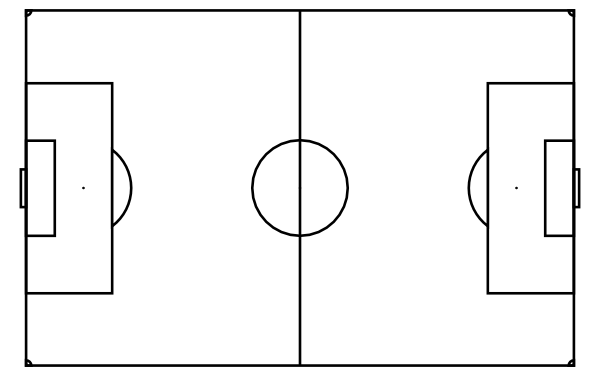
\includegraphics[scale=0.3]{../img/pitch.png}
\caption{Vzhľad futbalového ihriska, pre medzinárodné zápasy musí mať dlhšia strana 115 -- 120\,m, kratšia 64 -- 95\,m} 
\label{pitch}
\end{figure}

\subsection{Futbalové ligy}
Väčšina futbalových líg na svete (vrátane tých, s ktorými sa pracuje v tejto práci) funguje aspoň z časti sezóny na systéme, ktorý môžeme nazvať \textit{každý s každým}.
To znamená, že každý tím odohrá zápas proti každému tímu v lige.
Každá sezóna týchto líg sa najprv delí na kolá a až potom na zápasy.
V každom kole odohrá jeden zápas každý tím (s výnimkou jedného tímu, ak liga obsahuje nepárny počet tímov, ten má v danom kole voľno).
Za výhru v každom zápase sú 3 body, za remízu 1 bod a za prehru nedostane tím žiaden bod.
Sledované ligy fungujú na barážovom systéme, teda najnižšie umiestnené tímy zostupujú do nižšej ligy v hierarchii líg v danej krajine a najvyššie umiestnené tímy postupujú do vyššej ligy v hierarchii.

\section{Tenis}
Tenis je šport tímov súperiacich proti sebe, skladajúcich sa z jedného alebo dvoch ľudí, hrajúcich proti sebe na tenisovom kurte.
Zápasy sa delia na dvojhry, teda zápasy dvoch jednočlenných tímov, a štvorhry, zápasy dvoch dvojčlenných tímov.
Hlavným cieľom tenisu je použiť tenisovú raketu na zahratie loptičky na súperovu stranu kurtu (obrázok \ref{court}) jedným úderom tak, aby mala súperiaca strana, čo najväčší problém ho vrátiť naspäť \citep{tenis:kor}. 
Ak sa to jednému z tímov nepodarí v súlade s pravidlami, súper získa bod.
Tím, ktorý získa 4 body, získa hru. Ak obe tímy získajú po 3 body skôr, ako jeden z nich získa 4, hru získa tím, ktorý získa o 2 body viac ako súper.
Tím, ktorý skôr získa 6 hier, získa sadu. Ak nastane stav 5:5, hru získa tím, ktorý získa 7 hier.
Zápas sa hrá na dve alebo tri víťazné sady, toto číslo je vždy určené vopred.
V tejto práci nás budú hlavne zaujímať dvojhry, teda zápasy jeden proti jednému.
\citep{hry2}.

\noindent
\begin{figure} 
\centering
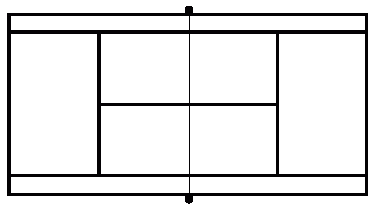
\includegraphics[scale=0.7]{../img/court.png}
\caption{Vzhľad tenisového kurtu, kurt je dlhý 23,77\,m, široký 10,97\,m, dodatočný prázdny priestor okolo kurtu je vyhradený, aby hráči mali možnosť dosiahnuť na loptičky, ktoré sú v hre, ale nachádzajú sa mimo kurtu. Sieť je vysoká 1.07\,m na krajoch kurtu, 0,91\,m v strede.}
\label{court}
\end{figure}

\subsection{Turnaje ATP Tour}
ATP Tour je tenisový okruh najvyššej celosvetovej úrovne organizovaný asociáciou ATP (Association of Tennis Professionals).
Profesionálni hráči sa schádzajú na turnajoch po celom svete.
Tieto turnaje sa hrajú vyraďovacím systémom, teda hráč ktorý vyhrá v zápase postúpi do ďalšieho kola turnaja až do finále.
Pár najvyšších hráčov postúpi priamo do vyraďovacej časti turnaja, ak sa doň prihlásia, zvyšní hráči ešte musia prejsť kvalifikáciou predtým, ako budú môcť hrať priamo na turnaji.
Turnaje spadajúce pod ATP Tour sú turnaje typu ATP Masters 1000, ATP 500 a ATP 250. Tieto turnaje sú nazvané podľa počtu bodov, ktoré si hráč pripíše za výhru.
Turnaje Grand Slam spadajú pod ITF (International Tennis Federation), víťaz ale za víťazstvo na týchto turnajoch dostane 2000 bodov.
ATP publikuje rebríček profesionálnych hráčov týždenne, hráči sú zoradení zostupne podľa počtu získaných bodov v poslednom roku.


\section{Porovnanie futbalu a tenisu}
Z predchádzajúcich kapitol je zrejmé, že futbal a tenis majú veľa spoločných a veľa rozdielnych vlastností. 
Futbal je kontaktný šport, teda protihráči sú často vo fyzickom kontakte medzi sebou, zatiaľ čo pri tenise sú protihráči vždy na opačných stranách tenisového kurtu. 
Rozdielny je aj počet hráčov v jednom tíme, vo futbale je maximálny počet hráčov hrajúcich v jednom momente za jeden tím 11, v tenise to je buď jeden alebo dvaja.
Spoločný je napríklad fakt, že sa jedná o loptový šport. 
Na druhej strane, vo futbale je povolené loptu zasiahnuť ktoroukoľvek časťou tela okrem rúk (s výnimkou brankára), v tenise je zakázané dotknúť sa tenisovej loptičky akoukoľvek časťou tela, loptičku je povolené zahrať len tenisovou raketou.
Ďalším rozdielom je hrací čas. Vo futbale má každý zápas fixnú dĺžku (2 polčasy po 45 minút s maximálne 15 minútovou prestávkou medzi nimi), rozhodca na konci každého polčasu nadstaví čas, po ktorý sa nehralo kvôli rôznym prerušeniam v hre 
\citep{hry1}.
V tenise môže zápas vďaka pravidlám trvať od desiatok minút do niekoľko hodín \citep{tenis:kor}.


\section{Kurzy stávkových na kancelárií}
Kurzové stávky sú stávky na akýkoľvek jav, na ktorý vypíše daná stávková kancelária kurz. 
Kurzy stanovuje bookmaker podľa toho, aká je pravdepodobnosť, že daný jav nastane, kde platí, že čím nižší kurz, tým je vyššia pravdepodobnosť nastania daného javu. 
Väčšinou sa tieto javy týkajú nejakej športovej udalosti, napríklad futbalových zápasov alebo automobilových pretekov. 
Stávkové kancelárie ale vypisujú kurzy aj na nešportové udalosti, kde medzi tie známejšie patria prezidentské voľby \citep{bet:pres} alebo ohlásenie mena novorodeného dieťaťa v kráľovskej rodine, kde zvyknú byť vypísané kurzy napríklad na pohlavie, meno novorodenca alebo presný dátum narodenia \citep{bet:prince}.

Na javy, na ktoré sú vypísané kurzy, môže potom zákazník staviť istú sumu peňazí, vklad, obvykle tak, že vloží tento vklad do stávkovej kancelárie. 
Ak daný jav nastane, zákazník dostane od tejto stávkovej kancelárie výhru, ktorá predstavuje výsledok vynásobenia daného kurzu vkladom.
Ak daný jav nenastane, vklad prepadá v prospech stávkovej kancelárie.
Pre príklad si vezmime tipovanie výsledku futbalového zápasu Slovensko - Česká republika, ktorý sa odohral dňa 13.10.2018. 
Podľa internetového portálu OddsPortal.com bol priemerný vypísaný kurz na tip domáci (v tomto prípade Slovensko) 2,06, na tip hostia (Česká republika) 3,86 a na tip remíza 3,35.
Zápas skončil výhrou hostí, čo znamená, že ak by sme boli stavili 100\,\rm korún na tento výsledok, tak by sme si boli odniesli zo stávkovej kancelárie 386\,\rm korún  (3,86 * 100 = 386), čo predstavuje zárobok 286\,\rm korún, pretože 100\,\rm korún predstavuje vklad.
Ak by sme boli stavili 100\,\rm korún na výhru domácich alebo na remízu, tak by sme boli prehrali celý vklad.

Stávkovanie je hazardná hra, obľúbená práve preto, že každý hráč môže vyhrať a vie aj ovplyvniť svoju pravdepodobnosť úspechu tým, že danú udalosť pozná \citep{odds}.

\begin{figure}
\centering
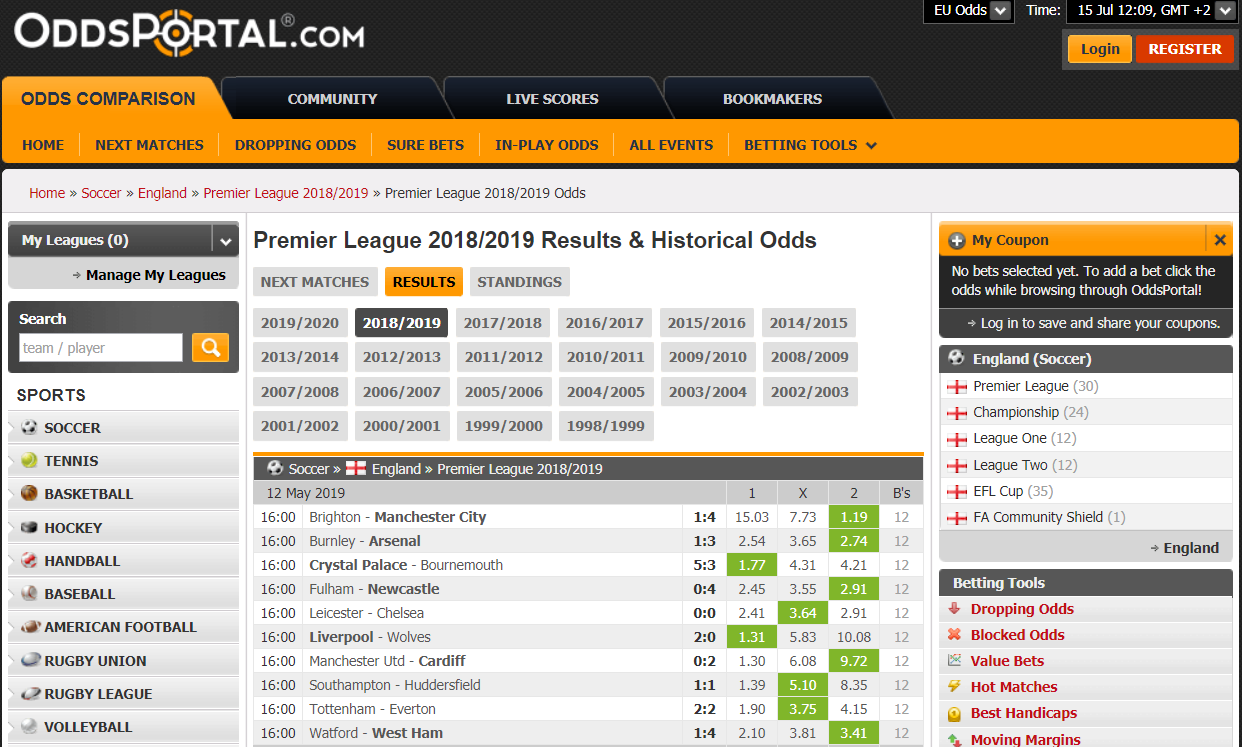
\includegraphics[width=\textwidth]{../img/odds.png}
\caption{Takto vyzerá stránka OddsPortal.com, z ktorej som získaval dáta pre potreby tejto práce. Znázornené je posledné kolo predikovanej časti anglickej \textit{Premier League}.} 
\label{odds}
\end{figure}
\chapter{Neurónové siete}

\iffalse
Formálne  je neurónová    sieť    určená    ako    orientovaný    graf    G=(V,E).    
Výrazy V={v1,v2,...,vN}  a  E={e1,e2,...eM}  označujú  neprázdnu  vrcholovú  množinu  resp.  hranovú množinu grafu G obsahujúceho N vrcholov (neurónov) a M hrán (spojov). Každý spoj $e \in E$ sa interpretuje ako usporiadaná dvojica dvoch neurónov z množiny V, e=(v,v’).  
Hovoríme, že  spoj  e  začína  v  neuróne  v  a  končí  v  neuróne  v’.  Množina  neurónov  V  je  rozložená  na disjunktné podmnožiny.

kde VI obsahuje NI vstupných neurónov, ktoré sú susedné len s vychádzajúcimi hranami, VH obsahuje NH skrytých (angl. hidden) neurónov, ktoré sú susedné súčasne  s  vychádzajúcimi ako aj s vchádzajúcimi hranami, a konečne VO obsahuje NO výstupných neurónov, ktoré súsusedné  len  s  vchádzajúcimi  hranami.  
V  našich  nasledujúcich  úvahách  budeme  vždy predpokladať,  že  množiny  VI  a  VO  sú  neprázdne,  t.j.  neurónová  sieť  obsahuje  vždy  aspoň jeden vstupný a jeden výstupný neurón.
Pre acyklické neurónové siete (ktoré neobsahujú orientované cykly neuróny môžu byť usporiadané do vrstiev VL  L  $LL=\cup \cup \cup \cup 12 3...t$, kde L1=VI je vstupná vrstva (obsahuje len vstupné neuróny), L2, L3,..., Lt–1 sú skryté vrstvya  Lt  je  výstupná  vrstva.  
Vrstva  Li  (pre  $1\leq i\leq t$)  je  určená  nasledujúcim  jednoduchým spôsobom $LVivdvi=\in   =+;aflq1$, kde vzdialenosť d(v) sa rovná dĺžke maximálnej cesty, ktorá spája daný neurón so vstupným neurónom, potom musí platiť d(v)=0, pre $v\in VI$. 
Neurónová sieť určená acyklickým grafom je  obvykle  volená  tak,  že  neuróny  z  dvoch  susedných  vrstiev  sú  poprepájané  všetkými možnými  spojmi.  
Žiaľ,  takýto  rozklad  množiny  neurónov  na  vrstvy  je Obrázok 5.2. 
Neurónová sieť je definovaná ako orientovaný súvislý graf. 
Diagram A obsahuje orientovaný graf  s  jedným  cyklom  a  teda  nemôže  byť  použitý  pre  definíciu  neurónovej  siete  s  dopredným  šírením.
Diagram  B  ilustruje  možnosť  rozkladu  vrcholov  (neurónov)  acyklického  orientovaného  grafu  na  vrstvy L1,..,L4.
kde L1=VI je vstupná vrstva (obsahuje len vstupné neuróny), L2, L3,..., Lt–1 sú skryté vrstvya  Lt  je  výstupná  vrstva.  Vrstva  Li  (pre  $1\leq i\leq t$)  je  určená  nasledujúcim  jednoduchýmspôsobom$LVivdvi=\in   =+$;aflq1                                  (5.9)kde vzdialenosťd(v) sa rovná dĺžke maximálnej cesty, ktorá spája daný neurón so vstupnýmneurónom, potom musí platiťd(v)=0, pre $v\in VI$. Neurónová sieť určená acyklickým grafomje  obvykle  volená  tak,  že  neuróny  z  dvoch  susedných  vrstiev  sú  poprepájané  všetkýmimožnými  spojmi  (pozri  obr.  5.3). \citep{rnn:spol}

\fi

%\iffalse
Neural networks are composed of nodes or units (see Figure 18.19) connected by directed links. 
A link from unit i to unit j serves to propagate the activation $a_i$ from i to j.
Each link also has a numeric weight $w_{i,j}$ associated with it, which determines the strength and sign of the connection. 
Just as in linear regression models, each unit has a dummy input $a_0=1$ with an associated weight $w_{0,j}$. 
Each unit j first computes a weighted sum of its inputs: $$in_j=\sum^n_{i=0}w_{i,j}a_i$$
Then it applies anactivation function g to this sum to derive the output: 
$$a_j=g(in_j)=g\left(\sum^n_{i=0}w_{i,j}a_i\right)$$

The activation function $g$ is typically either a hard threshold (Figure 18.17(a)), in which case the unit is called a perceptron, or a logistic function (Figure 18.17(b)), in which case the term sigmoid perceptron is sometimes used.  Both of these nonlinear activation function ensure the important property that the entire network of units can represent a nonlinear function (seeExercise 18.22). As mentioned in the discussion of logistic regression (page 725), the logistic activation function has the added advantage of being differentiable. Having decided on the mathematical model for individual “neurons,”  the next task is to connect them together to form a network.  There are two fundamentally distinct ways to do this.  

A feed-forward network has connections only in one direction—that is, it forms a directed acyclic graph. Every node receives input from “upstream” nodes and delivers output to “downstream” nodes; there are no loops. A feed-forward network represents a function of its current input; thus, it has no internal state other than the weights themselves. 

A recurrent network,  on  the  other  hand,  feeds  its  outputs  back  into  its  own  inputs.   This  means  that the activation levels of the network form a dynamical system that may reach a stable state or exhibit oscillations or even chaotic behavior. Moreover, the response of the network to a given input depends on its initial  state,  which may depend on previous inputs.  Hence,  recurrent networks (unlike feed-forward networks) can support short-term memory.  This makes them more interesting as models of the brain, but also more difficult to understand.

Feed-forward networks are usually arranged in layers, such that each unit receives input only from units in the immediately preceding layer. In the next two subsections, we will look at single-layer networks, in which every unit connects directly from the network’s inputs to its outputs, and multilayer networks, which have one or more layers of hidden units that are not connected to the outputs of the network. 


%\fi

\section{Popredné neurónové siete}

\section{Rekurentné neurónové siete}
Vo  všeobecnosti  možno  za  rekurentnú  sieť  považovať akúkoľvek  neurónovú  sieť,  v  ktorej  istá  podmnožina  neurónov  (rekurentné  neuróny)  jes chopná  uchovať  informáciu  o  svojich  aktiváciách  v  predošlých  časoch  pre  výpočet aktivácií  neurónov  v  čase t+1.  “Odpamätané”  hodnoty  sa  objavia  v  čase t+1  ako  aktivácie tzv. kontextových   neurónov \citep{rnn:spol}
\chapter{Datasety}

Data, s ktorými budeme pracovať, sú výhradne len výsledky a konečné stavy jednotlivých zápasov. 

\section{Futbal} \label{foot}
Pre futbal získame všetky zápasy sezóny pre danú ligu. 
Musia byť všetky, pretože v ďalšej časti sa počíta na základe už odohraných zápasov a jeden zápas by mohol skresliť výsledky. 
Jednotlivé ligy boli teda vyberané nielen na základe kvality, ale aj na základe toho, že v pár posledných sezónach sa ani raz nestalo, že zápas musel byť z nejakého hľadiska udelený kontumačne jednému z tímov (ako sa napríklad stalo vo francúzskej lige v roku 2007 pre problémy s divákmi \citep{awarded}) alebo celá sezóna bola poznačená korupčným škandálom ako v prípade talianskej ligy v sezóne 2006 \citep{scandal}.
Takéto výsledky by nemuseli skresliť stavbu neurónovej siete, ale všeobecne je lepšie, ak sa takýmto situáciám vyhneme.

Data pre každú ligu predstavujú výsledky všetkých zápasov odohraných len vrámci ligy za pár posledných sezón. 
Nebudeme používať žiadne data informujúce o hráčoch, ktorí sú v oficiálnej súpiske na zápas ani data o základnej zostave na daný zápas a ani ďalšie informácie o priebehu zápasu ako percentuálne držanie lopty alebo počet striel, či rohových kopov.
Taktiež vzhľadom na to, že tímy v jednotlivých ligách hrajú zápasy aj mimo ligy, prinajmenšom zápasy v ligovom pohári, tak nebudú použité ani informácie o oddychu pred daným zápasom, teda koľko dní pred zápasom mali zúčastnené tímy voľno.

Dataset pre každú ligu je tabuľka, kde riadky predstavujú jednotlivé zápasy zoradené podľa dátumu, v ktorom bol zápas odohraný, zostupne.
Stĺpce sú v poradí:
\begin{enumerate}
  \item Jednoznačný názov domáceho tímu (nemusí byť celý názov, stačí skrátený, ale jednoznačný a, pokiaľ možno, v celom datasete konzistentný),
  \item Jednoznačný názov hosťujúceho tímu,
  \item Identifikátor zápasu,
  \item Ligové kolo, v ktorom sa zápas odohral (0, ak sa nevie),
  \item Identifikátor domáceho tímu,
  \item Identifikátor hosťujúceho tímu,
  \item Počet gólov strelených domácim tímom v zápase,
  \item Počet gólov strelených hosťujúcim tímom v zápase,
  \item Dátum zápasu,
  \item Sezóna,
  \item Kurz na výhru domácich,
  \item Kurz na remízu,
  \item Kurz na výhru hostí.
\end{enumerate}

Posledné 3 stĺpce teda predstavujú kurzy na dané výsledky. Tieto ale nie sú pri trénovaní siete využívané, a teda pre dáta, ktoré sú vždy použité len pre trénovanie ani nie sú vyžadujúce.

\noindent
\begin{figure}[b]
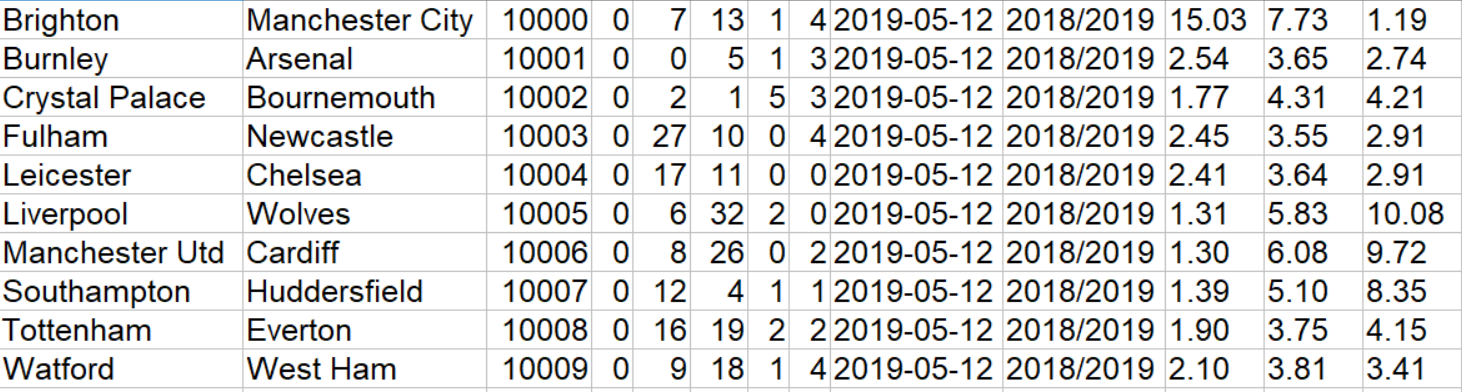
\includegraphics[width=\textwidth]{../img/eng.png}
\caption{Ukážka prvých 10 riadkov z tabuľky všetkých zápasov anglickej Premier League ilustrujúcich členenie tabuľky}
\end{figure}
dáta v trénovacom súbore obsahuje prvú polovicu sezóny 2018/2019 a 7 jej celých predchádzajúcich sezón. Prvá polovica sezóny predstavuje všetky odohrané zápasy od začiatku sezóny až po odohratie posledného zápasu pred začiatkom kola, ktoré je numericky už v druhej polovici sezóny. 
Napríklad najvyššia anglická futbalová liga, Premier League, má 38 kôl každú sezónu, do úvahy sa bude brať posledných 7 sezón pred sezónou 2018/2019 a všetky zápasy odohrané pred prvým zápasom 20. kola sezóny 2018/2019 (s výnimkou predohrávok, teda zápasov, ktoré boli preložené na dátum pred dátumom, v ktorom daný zápas figuroval v predsezónnom rozpise zápasov).


\subsection{Motivácia pre výber daných príznakov}
Vybrané príznaky presne popísané v sekcii Prílohy (Príloha \ref{in:foot}) sa dajú rozdeliť viacerými spôsobmi do skupín.
Medzi danými príznakmi sa ešte budú selektovať tie najdôležitejšie v jednej z nasledujúcich sekcii (konkrétne sekcia \ref{stavba}).

Prvým spôsobom je rozdeliť tieto príznaky tak, ako za sebou nasledujú do skupiny po desiatich. To nám vytvorí 5 skupín, môžeme ich po poradí nazvať príznaky sezóny, roly, formy, vzájomných zápasov a doplnkové.
Skupina príznakov sezóny obsahuje dáta o celom doterajšom priebehu sezóny pre obe tímy. Tieto dáta sú z môjho pohľadu dôležité. Mohlo by byť dôležité vedieť, ako daný tím vystupuje v celej sezóne.

Príznaky roly obsahujú dáta o výsledkoch daných tímov v role, v akej sa predstavia v predikovanom zápase (domáci alebo hostia) počas celej sezóny. To by mohlo byť dôležité, pretože je rozdiel v zápasoch, kde tímy hrajú doma a v zápasoch, kde hrajú vonku. Tento rozdiel je individuálny. Tím môže vyhrávať napríklad len na domácom ihrisku a mimo neho sa im nemusí až tak dariť, v tom prípade by v role hostí nemuseli byť favoritom na víťazstvo, aj keď by to mohla predchádzajú skupina očakávať.

Tretia skupina je forma, hodnotených je posledných 5 zápasov, tradične to v predikovaných ligách predstavuje obdobie 4 -- 5 týždňov, viac už by nemuselo toľko hovoriť o forme daného tímu, je dosť času stratiť, respektíve znovu získať psychickú pohodu. Forma by mala byť dôležitá, pretože určuje, ako sa tímu darilo v lige v posledných zápasoch, teda niečo ako psychickú pohodu tímu, s ktorou vstupuje do zápasu.

Príznaky vzájomných zápasov určujú posledných 5 vzájomných zápasov, ktoré dané tímy odohrali pred predikovaným zápasom. Prvých 5 príznakov sa týka celkových 5 vzájomných zápasov, ďalších 5 sa týka vzájomných zápasov odohraných na ihrisku domáceho v predikovanom zápase. Každý tím hrá iný štýl hry a každý štýl funguje lepšie proti nejakému štýlu a horšie zas proti inému štýlu (to bol jeden z výsledkov vo vyššie spomínanom článku \citep{related:shin}). Tímy svoje štýly nezvyknú meniť veľmi často, pretože obvykle by na to potrebovali aj výmenu hráčov. Cieľom týchto príznakov je ohodnotiť, ako sa darí daným tímom, keď sa stretnú medzi sebou.

Poslednou skupinou sú zvyšné príznaky určené na trénovanie, a to je dlhodobá sila domáceho a hosťujúceho mužstva a skóre. 
Niekedy sa môže stať, že tím mal ťažký úvod do sezóny, ale z minulých sezón vieme, že sa im v lige darí obvykle oveľa lepšie a môžeme očakávať, že v nasledujúcich zápasoch začnú uhrávať lepšie výsledky. 
To je dôvodom výberu dlhodobej sily mužstva do skupiny príznakov.
Je to najbližšie ako sa môžeme dostať ku abstraktnému ohodnoteniu kvality mužstva, ktoré používali moji predchodcovia (ako napríklad Shin a Gasparyan v \citep{related:shin}) z reálnych dát.

Skóre je pokus ohodnotiť formu tímu jedným údajom čo najlepšie.
Čím väčší počet vstupných neurónov, tým viac dimenzií dodávame neurónovej sieti.
S väčším počtom dimenzií rastie objem celkového priestoru, a to znamená, že sa jednotlivé body dát od seba oddeľujú a samotné dáta sa stávajú redšie.
Tomuto fenoménu hovoria vedci kliatba dimenzionality (\citep{curse}).
Práve kvôli tomu som sa pokúsil vytvoriť umelé príznaky, ktoré by mohli ohodnotiť rozdiel formy oboch tímov v jednom údaji, na rozdiel od desiatich (popísané sú v Prílohe \ref{in:foot} 44 a 45, detailnejšie pod zoznamom).

Každá z prvých 4 skupín obsahuje dvakrát 5 rôznych údajov, z ktorých môžeme opäť spraviť päť skupín príznakov, a to víťazstvá, remízy, prehry, priemerný počet strelených gólov a priemerný počet inkasovaných gólov.

Prvé tri tieto skupiny hovoria samé za seba, snažíme sa predikovať výsledok zápasu, ktorý je buď výhra, remíza alebo prehra z hľadiska oboch tímov. Zvyšné dve skupiny sa snažia z daných dát simulovať niečo ako ofenzívnu a defenzívnu silu mužstva, podobne ako robili moji predchodcovia (napríklad \citep{related:igiri}).

\section{Tenis} \label{ten}
Pre tenis získame všetky zápasy každého turnaja ATP typu 500, 1000 a Grand Slam, kde hraje aspoň jeden hráč z Top 100 rebríčka ATP pre danú sezónu.
Dôvodom je fakt, že predikujeme zápasy týchto turnajov medzi hráčmi z Top 100 rebríčka ATP, ale pre týchto hráčov počítame ich momentálnu formu, takže sú pre nás dôležité aj zápasy, ktoré odohrajú proti hráčom, ktorí sa nenachádzajú v Top 100.
Fakt, že množstvo hráčov z Top 100 sa pravidelne zúčastňuje turnajov typu ATP 250, určuje, že niekedy nastúpia dvaja takíto hráči aj proti sebe na takomto turnaji. Vďaka tomu a aj relatívnej kvalite týchto turnajov som sa rozdodol, že tieto turnaje zoberieme do úvahy (vzájomné zápasy medzi jednotlivými hráčmi na takto ohodnotených turnajoch tiež patria medzi údaje, z ktorých sa stávajú vstupné neuróny (ako vidieť v Prílohe \ref{in:ten})). 

V tenise sa nemôžeme vyhnúť zápasom, ktoré boli nejakým spôsobom udelené jednému z hráčov, či už bez boja alebo po skreči súpera v priebehu zápasu, pretože zranenia sú súčasťou profesionálneho športu.
Vo futbale sa to obvykle rieši prestriedaním zraneného hráča, v tenise to, prirodzene, nie je možné.
Pre potreby tejto práce máme dve možnosti, buď môžeme tieto zápasy úplne ignorovať alebo ich môžeme započítavať do niektorých oblastí vstupu (ako napríklad forma alebo vzájomné zápasy) a ignorovať inde (predpovedať takéto výsledky je možno nápad pre inú prácu). 
Pre potreby tejto práce budeme tieto zápasy úplne ignorovať, čo znamená, že sa nevyskytnú v trénovacích ani testovacích dátach.
Samozrejme, má to svoje výhody aj nevýhody.
Výhodou je, že výsledky budú reálne odzrkadľovať presnosť siete na zápasoch, ktoré sa odohrali a skončili.
Predpovedať zranenie totiž nepatrí medzi ciele tejto práce.
Ďalšou výhodou je spravodlivosť oblastí vstupu ako forma a vzájomné zápasy, pretože sa tam berú len zápasy, ktoré sa dohrali do konca, takže tieto čísla sa v žiadnom okamihu nenafukujú. Ak by napríklad hráč natrafil počas turnaja na dvoch/troch súperov, ktorí sa vzdajú, tak by sa mu vo forme ukázali tieto víťazstvá, aj keď to neboli plnohodnotné výhry.
Nevýhodou je, že výsledky nemusia ukazovať reálne výsledky v praxi (pred zápasom nevieme určiť, či sa hráč zraní, ale sieť aj tak vydá svoju predpoveď, aj keď nebola na tieto údaje trénovaná).

dátaset je tabuľka, každý zápas predstavuje jeden riadok tabuľky, zápasy sú zoradené do turnajov od najskôr odohraných turnajov po tie najbližšie súčasnosti (ak sa obe turnaje začali a končili hrať v rovnaký deň, tak sú v ľubovoľnom poradí, nie je možné, aby poradie zmenilo nejaké dáta, pretože nie je možné hrať na dvoch turnajoch takéhoto typu zároveň). 
Zápasy v turnajoch sú zoradené od finále po prvé kolo, teda intuitívne opačne. Program v transformačnej časti si už to poradie upraví, aby zápasy nasledovali chronologicky. 
Stĺpce tabuľky sú v poradí:
\begin{enumerate}
  \item Názov turnaja,
  \item Počet bodov, ktoré víťaz obrdží za výhru v turnaji (ak to je neznáme, tak je tam nápis N/A)
  \item Rok, v ktorom sa turnaj odohral,
  \item Povrch kurtov na turnaji (tvrdý \textit{(Hard)}, antukový\textit{(Clay)} alebo trávnatý povrch \textit{(Grass)}),
  \item Meno víťaza zápasu,
  \item Meno hráča, ktorý zápas prehral,
  \item Kolo turnaja, v ktorom sa zápas odohral od najdôležitejšieho (1 značí finále, 2 semifinále, apod.),
  \item ID zápasu,
  \item ID víťaza*,
  \item ID porazeného hráča*,
  \item Počet setov, ktoré v zápase získal víťaz,
  \item Počet setov, ktoré v zápase získal porazený hráč,
  \item Počet hier, ktoré v zápase získal víťaz v jednotlivých setoch oddelené znakom |,
  \item Počet hier, ktoré v zápase získal porazený hráč v jednotlivých setoch oddelené znakom |,
  \item Predzápasový kurz na výhru víťaza zápasu,
  \item Predzápasový kurz na výhru porazeného hráča v zápase.
\end{enumerate}
* - ak je ID hráča NULL, znamená to, že hráč sa doposiaľ ani raz neumiestnil v Top 100 rebríčka ATP

Postavenia hráčov v rebríčku ATP sú získané z pomocného súboru (ukážku z tohto súboru je možné vidieť na obrázku \ref{rank}). Tam sú uchovávané, súbor v transformačnej vrstve práce si pospája hráčov s ich id a ich umiestnením v práve vyhodnocovanom roku.

\noindent
\begin{figure}[b]
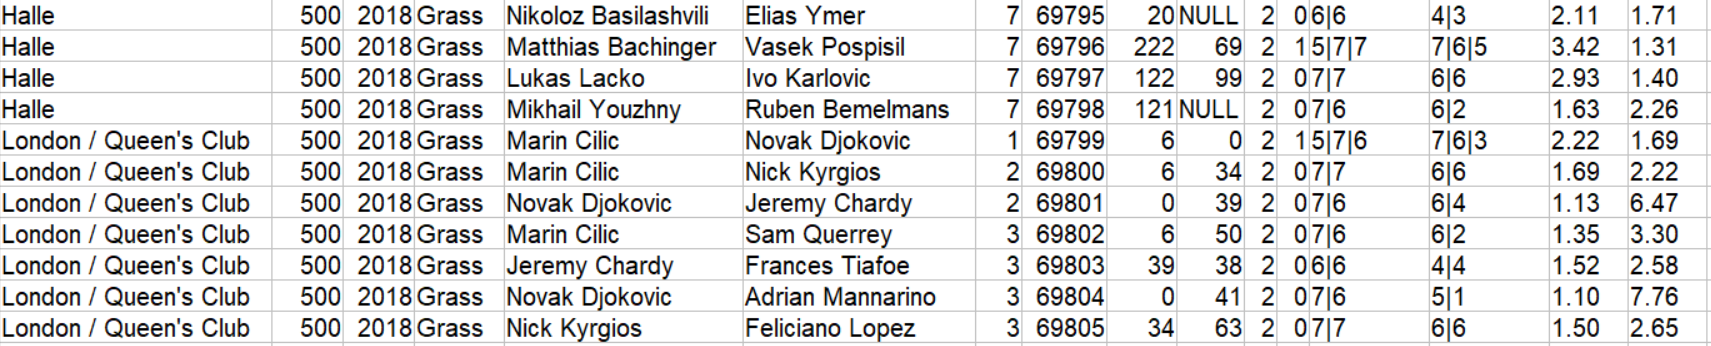
\includegraphics[width=\textwidth]{../img/atp.png}
\caption{Ukážka vybraných pár riadkov z tabuľky zápasov v okruhu ATP ilustrujúcich stĺpce a riadky.}
\end{figure}

\noindent
\begin{figure}
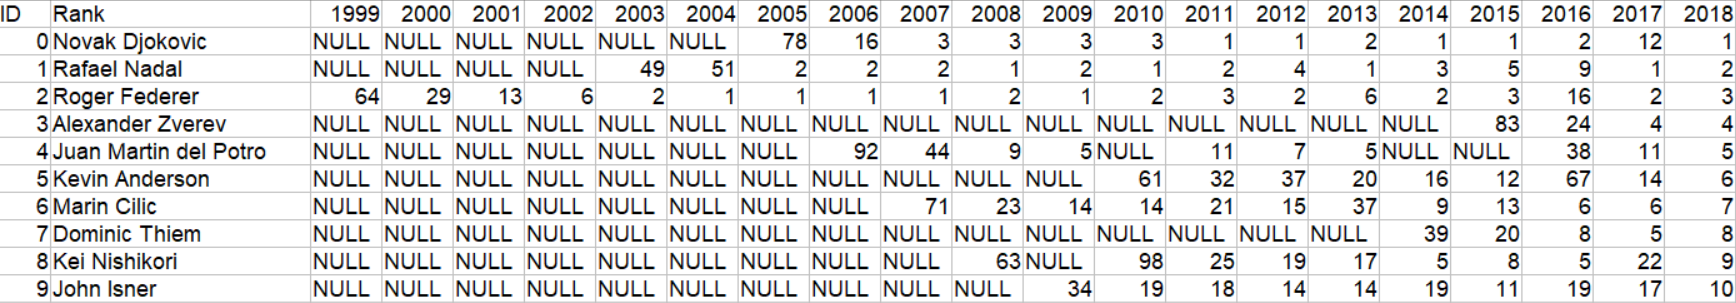
\includegraphics[width=\textwidth]{../img/rank.png}
\caption{Ukážka prvých 10 riadkov spolu aj s hlavičkou z pomocného súboru udržiavajúceho postavenie hráčov v rebríčku ATP. Hodnota \textit{NULL} znamená, že sa hráč na konci daného roku neumiestnil v prvej 100 rebríčka.}
\label{rank}
\end{figure}

\subsection{Motivácia pre výber daných príznakov}
Podobne ako pri futbale si môžeme jednotlivé príznaky zhrnúť do skupín a jednotlivé skupiny predstaviť. Význam jednotlivých príznakov je vypísaný v Prílohe (Príloha \ref{in:ten}).

Najprv si môžeme tieto príznaky rozdeliť na skupinové (prvých 30) a jednotlivé.
Na skupinové sa môžeme najprv pozrieť ako na skupiny po 6, a to príznaky roku, formy, povrchu, formy na povrchu a vzájomných zápasov.

Príznaky roku určujú, ako sa danému hráčovi darilo v danom kalendárnom roku.
Táto kategória má zväčša najvyššie hodnoty zo všetkých skupín. Tieto údaje je dôležitejšie v neskorších fázach roka, ukazujú všeobecný obraz o celom ročníku.

Príznaky formy ukazujú, ako sa hráčovi darilo v posledných 10 zápasoch. Na rozdiel od futbalu sa tieto dáta prenášajú z roka na rok, takže ak hráč ukončil rok dvakrát po sebe v Top 100 rebríčka ATP počas sledovaných sezón, tak na začiatku druhého roku sa mu ukáže forma aj z minulého roku. Je to tak vyriešené preto, lebo tenis sa hraje v podstate celý rok narozdiel od futbalu, kde liga zvykne končiť v máji a začínať v auguste a počas tejto doby sa môžu udiať zmeny v tíme.
Dôležité z podobného dôvodu ako pri futbale, ukazujú momentálnu výkonnosť a psychickú pohodu hráča, s ktorou prišiel do zápasu.

Príznaky povrchu ukazujú, ako hral hráč na povrchu, na ktorom odohrá predikovaný zápas, počas roka. V tenise majú rôzne povrchy rôzne vlastnosti. Každý hráč má svoj preferovaný povrch, kde sa mu hrá najlepšie alebo dosahuje najlepšie výsledky. Tieto príznaky celkovú výkonnosť daného hráča na tomto povrchu v doterajšom priebehu sezóny.

Príznaky formy na povrchu predstavujú kombináciu oboch predošlých skupín, formy a povrchu. Uchováva údaje o posledných 10 zápasov odohraných na danom povrchu, dáta sa prenášajú cez rok. Dôvody sú dva, prvým je, že obvykle sa rok začína a aj končí na tvrdom povrchu a druhým dôvodom je psychika hráča. Aj keď hráč nehral skoro celý rok na danom povrchu, jeho podvedomie si určite pamätá, ako sa mu tam darilo naposledy, aj na základe toho sa môže tešiť alebo netešiť na zápasy na danom povrchu.

Poslednú skupinu v tomto pohľade predstavujú príznaky vzájomných zápasov, tie sa ešte delia na dve skupiny, všetky vzájomné zápasy a vzájomné zápasy odohrané na povrchu, na ktorom sa bude hrať predikovaný zápas. 
Tieto príznaky by som považoval možno aj za tie najdôležitejšie, ak majú hráči dostatočnú históriu vzájomných zápasov.
Každý hráč má vlastný štýl a proti niektorým štýlom sa mu hraje lepšie ako proti iným. Naviac, narozdiel od futbalu, tenisti za celú svoju kariéru nezvyknú radikálne meniť svoje štýly hry, takže tieto údaje sú relevantné aj po rokoch.
Tieto údaje sú uvedené z pohľadu hráča 1.

Každá táto skupina má údaje o hráčovi 1 a hráčovi 2 v zápase a obsahuje 3 údaje pre každého hráča, počet výhier, prehier a priemerný rozdiel v počte vyhraných a prehraných hier za set. Prítomnosť prvých dvoch je zjavná, snažíme sa predikovať buď výhru alebo prehru. 
Prítomnosť poslednej je tu ako pokus o ukážku sily hráča. 
Teória za tým je taká, že sa môže stať, že hráč narážal počas turnaja na hráčov, s ktorými v zápase vyhrával jednoznačne a potom prišiel zápas, kde prehral, ale bol to vyrovnaný zápas. 
Takýto hráč sa potom môže stretnúť s hráčom, ktorý má podobné výsledky, ale ak vyhral, tak to bol tesný zápas a ak prehral, tak prehral jednoznačne.
Pri predikcii výsledku tohto zápasu by bol pravdepodobne favorizovaný prvý hráč, ale ak by sme tento údaj nemali a ostatné údaje by boli dostatočne podobné, tak by mohla mať sieť problémy s rozhodovaním.

Jednotlivé príznaky sú umiestnenia oboch hráčov v poslednom koncoročnom rebríčku ATP, kategorizácia povrchu a skóre.
Postavenie hráča v poslednom koncoročnom rebríčku ATP ukazuje, ako sa darilo hráčovi v poslednom roku (keďže rebríček uchováva body z posledného roka). Niečo, na čo sa môžeme odvolávať hlavne na začiatku ročníka, keď je ešte málo údajov v tohto roka.

Kategorizácia povrchu je skupina príznakov, ktorá je prítomná hlavne z dôvodu, že pre rôzne povrchy môže fungovať iné ohodnotenie. Napríklad na tvrdom povrchu by sa kládol dôraz na iné aspekty ako na trávnatom povrchu.

Skóre je pokus ohodnotiť formu hráča výraznejšie ako len počtom výhier a prehier. Pri pokusoch a vylaďovaní siete budeme v kapitole Stavba siete (kapitola \ref{stavba}) selektovať dané vstupné neuróny podľa rôznych kritérií a vyskúšame tiež aj ako sa bude sieť správať, ak nahradíme všetky stĺpce obsahujúce dáta o forme rozdielom v skóre.
Teoreticky by sme tým mohli ušetriť 4 vstupné neuróny (forma obsahuje 6 príznakov, ale skóre sa delí na dva príznaky, obe presne popísané v Prílohe \ref{in:ten}).
\chapter{Stavba siete} \label{stavba}

Všetky siete boli napísané v programovacom jazyku \textit{Python} s použitím knižníc \textit{numpy} a \textit{tensorflow}.
V prípade futbalu bola na začiatku sieť skonštruovaná so všetkými 44 príznakmi, ktoré sme dostali z transformačnej časti práce (Príloha \ref{in:foot}).
Sieť teda obsahovala vstup o veľkosti 44 príznakov, 2 skryté vrstvy neurónov (s 25, resp. 15 neurónmi) a troj-neurónový výstup typu softmax, ktorý vyberie najpravdepodobnejšiu možnosť, nastaví daný výstup neurónu na 1 a zvyšné nastaví na 0.
V prípade tenisu bola sieť skonštruovaná so všetkými 37 príznakmi (ich popis je Príloha \ref{in:ten}) a taktiež obsahovala 2 skryté vrstvy neurónov s rovnakým počtom neurónov na nich ako v prípade futbalu. Výstup predstavoval dva neuróny, na ktoré bol opäť použitý softmax, ktorý vyberie najvyššiu hodnotu.
Na vylepšovanie siete sme, ako je napísané v jednej z predošlých kapitol (\ref{docu}), použili údaje, ktoré sa napokon budú pri vyhodnocovaní nachádzať medzi testovacími datami. 

Konkrétne, pre futbal data predstavovali 7 celých sezón a prvú polovicu ďalšej sezóny (ako popísané v \ref{foot}), vyhodnocovacie data predstavujú teda druhú polovicu tejto sezóny. 
Takže sme trénovacie data rozdelili na tri časti, 6 celých sezón a polovicu ďalšej (trénovacie data), druhú polovicu siedmej sezóny (testovacie data) a zvyšnú prvú polovicu ôsmej sezóny (nepoužité data).
V prípade tenisu prišli data už priamo z transformačnej časti v troch súboroch, trénovacie, testovacie a vyhodnocovacie data.

Každá sieť mala svoje nedostatky v celkovej úspešnosti, ale doposiaľ neexistuje efektívne nastavenie neurónových sietí pre každú situáciu \citep{gitgud}, takže každá sieť sa musela vylepšovať osobitne a manuálne vzhľadom na rozdiely v prístupoch.
Cieľom práce nie je porovnať rovnakú architektúru a viac typov neurónových sietí, ale pokúsiť sa získať, čo možno najlepšie výsledky a porovnať potenciály doprednej a rekurentnej neurónovej siete.

\section{Selekcia príznakov}
Kliatba dimenzionality nám hovorí, že čím viac vstupných príznakov zadáme neurónovej sieti, tým sú data redšie a teda je ich potreba získať viac, aby sa sieť správne učila. Viac dat získať nevieme, takže sa pokúsime znížiť počet dimenzií a pozrieť sa na to, ako sa to prejaví na trénovacích datach.
Na začiatok spravíme korelačný test všetkých príznakov testovacích a trénovacích dat (obrázky \ref{corr} a \ref{corr_atp}).
Teória hovorí, že by nám mohla napovedať, aké hodnoty sú dôležité.
Obrázok hovorí, že najvyššiu koreláciu s výsledkom zápasu majú príznaky 41 a 42 určujúce dlhodobú silu tímu. Skóre dosahuje tiež celkom vysokú koreláciu (okolo 0,2) s finálnym výsledkom.
V prípade tenisu obrázok naznačuje najvyššiu koreláciu medzi výsledkom a oboma druhmi skóre, veľkú rolu zohráva postavenie v rebríčku ATP a vzájomné zápasy (konkrétne priemerný rozdiel v počte vyhraných gemov za set).

\noindent
\begin{figure} \label{corr}
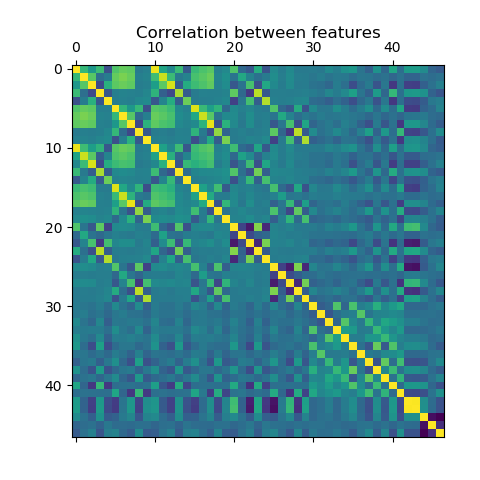
\includegraphics[scale=0.9]{../img/correng.png}
\caption{Korelačná tabuľka všetkých príznakov pre anglickú Premier League, žltá predstavuje kladnú koreláciu, modrá zápornú. Nás hlavne zaujímajú posledné 3 riadky určujúce koreláciu príznaku s výsledkom zápasu (príznaky sú v poradí ako v Prílohe \ref{in:foot}).}
\end{figure}
\begin{figure} \label{corr_atp}
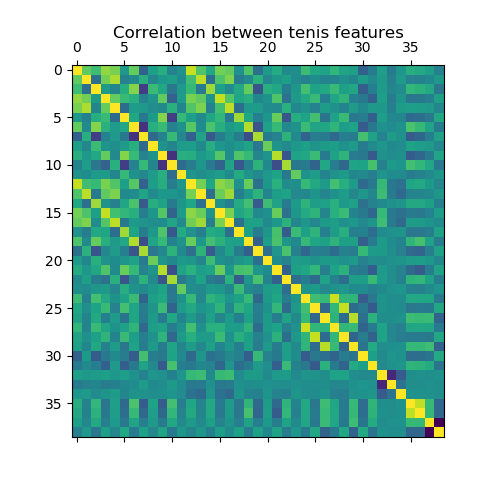
\includegraphics[scale=0.9]{../img/corratp.png}
\caption{Korelačná tabuľka všetkých príznakov pre tenisové zápasy, žltá predstavuje kladnú koreláciu, modrá zápornú. Nás hlavne zaujímajú posledné 2 riadky určujúce koreláciu príznaku s výsledkom zápasu (príznaky sú v poradí ako v Prílohe \ref{in:foot}).}
\end{figure}

Tieto tabuľky boli pre nás viac-menej informačné. 
Selekcia príznakov, s ktorými dosahovala sieť najlepšie trénovacie výsledky a ktoré budú použité na získanie výsledkov v kapitole \ref{res}, bol uskutočnený spôsobom pokus-omyl, keďže nič lepšie nevieme, ako už bolo spomínané na začiatku kapitoly.

\section{Výsledky tréningu}
Pri trénovaní siete boli pre každú množinu príznakov prenastavované aj iné parametre siete, pri snahe získať čo najlepšie výsledky.
Iba pre tréning doprednej neurónovej siete na predikciu futbalu predstavoval viac ako 100 rôznych vyskúšaných modelov siete, celkový počet vyskúšaných modelov bol okolo 250.
Tabuľky \ref{ff_train_res} a \ref{rnn_train_res} predstavujú nastavenia jednotlivých parametrov siete, pri ktorých dosahovali dopredné, resp. rekurentné neurónové siete najlepšie výsledky.

\begin{table}[h]
\begin{center}
\begin{tabular}{ p{7em}|c|c|c|c|c|c|c|c|c|c| } 
 Predpovedaný šport (liga) & \multicolumn{6}{|c|}{Parametre siete} & \multicolumn{4}{|c|}{Trénovacie výsledky}  \\ 
 \hline
  & O & B & LR & E & $H_1$ & $H_2$ & TrA\% & TeA\% & CG\% & CGP \\
 \hline \hline
 0 & 0 & 0 & 0 & 0 & 0 & 0 & 0 & 0 & 0 & 0 \\ 
 0 & 1 & 1 & 0 & 0 & 0 & 0 & 0 & 0 & 0 & 0 \\ 
 1 & 0 & 1 & 0 & 0 & 0 & 0 & 0 & 0 & 0 & 0 \\ 
 1 & 1 & 0 & 0 & 0 & 0 & 0 & 0 & 0 & 0 & 0 \\ 
 \hline
\end{tabular}
\caption{Tabuľka funkcie XOR}
\label{ff_train_res}
\end{center}
\end{table}

\begin{table}[h]
\begin{center}
\begin{tabular}{ p{7em}|c|c|c|c|c|c|c|c|c|c|c|c| } 
 Predpovedaný šport (liga) & \multicolumn{8}{|c|}{Parametre siete} & \multicolumn{4}{|c|}{Trénovacie výsledky}  \\ 
 \hline
  & O & B & LR & E & $H_1$ & $H_2$ & N & T & TrA\% & TeA\% & CG\% & CGP \\
 \hline \hline
 0 & 0 & 0 & 0 & 0 & 0 & 0 & 0 & 0 & 0 & 0 & 0 & 0 \\ 
 0 & 1 & 1 & 0 & 0 & 0 & 0 & 0 & 0 & 0 & 0 & 0 & 0 \\ 
 1 & 0 & 1 & 0 & 0 & 0 & 0 & 0 & 0 & 0 & 0 & 0 & 0 \\ 
 1 & 1 & 0 & 0 & 0 & 0 & 0 & 0 & 0 & 0 & 0 & 0 & 0 \\ 
 \hline
\end{tabular}
\caption{Tabuľka funkcie XOR}
\label{rnn_train_res}
\end{center}
\end{table}


\chapter{Dokumentácia} \label{docu}

Z programátorského hľadiska je práca rozdelená na tri časti. 
Prvú časť predstavuje získavanie výsledkov a kurzov jednotlivých zápasov. 
Druhú časť práce predstavuje transformácia dat na údaje priamo použiteľné pri konštrukcii neurónových sietí.
Poslednú časť tvorí stavba daného typu neurónovej siete pre daný šport.

Transformačná časť v prípade tenisu rozdelí data na 3 časti, trénovacie data, testovacie data (pre optimalizovanie siete) a vyhodnocovacie data.
V prípade futbalu data rozdelí na 2 časti, trénovacie a vyhodnocovacie data.
Pre optimalizáciu som použil program podobný programu v poslednej časti, ktorý si trénovacie data rozdelíl podľa potreby (konkrétne na prvých 6 celých sezón a prvú polovicu ďalšej a druhú časť tvorí druhá polovicu tejto sezóny, až následne prebiehalo učenie siete).
Je teda zaručené, že žiadna sieť neuvidí vyhodnocovacie data vopred pred finálnym vyhodnocovaním.
Vyhodnocovacie data sú použité až pre získavanie výsledkov použitých v tejto práci, a teda použili sa až v poslednej fáze.


Údaje, ktoré sa objavia vo výstupe sú celková úspešnosť a celkový zisk, úspešnosť a zisk siete pri vyrovnaných zápasoch (a vyrovnaný zápas považujem zápas, kde kurzy na výhru jedného alebo druhého tímu sa líšia najviac o 1) a úspešnosť a zisk siete pri výhradnom tipovaní zápasov, na ktoré máme istú dôveru (od hodnoty, ktorá je počítaná ako rozdiel dvoch najvyšších čísel, ktoré sieť vydá na výstup, jednoducho povedané, rozdiel najpravdepodobnejšej a druhej najpravdepodobnejšej možnosti výsledku zápasu z hľadiska siete).
Táto hodnota dôvery bola tiež vyoptimalizovaná pre každú sieť/program osobitne.


\section{Futbal}

Údaje o týchto zápasoch sa dajú stiahnuť jednoducho, spustením programu oddscaper.py a zadaním skratky danej ligy pre futbal ako parameter.
Skratky sú:
\begin{enumerate}
\item ENG - najvyššia anglická liga (Premier League)
\item GER - najvyššia nemecká liga (Bundesliga)
\item SPA - najvyššia španielska liga (La Liga)
\end{enumerate}
Program stiahne všetky výsledky a kurzy pre všetky zápasy všetkých kompletných sezón tej-ktorej ligy zo stránky www.oddsportal.com.

Tento dataset potom predáme programu \textit{DataMaker.exe} (TODO!) písanom v jazyku C\#, ktorý pretransformuje tieto data na vstupné neuróny pre neurónovú sieť. Všetkých vstupných neurónov je 44, ich význam a poradie je popísané v sekcii Prílohy (\ref{in:foot}). Program taktiež vydá ako posledné tri stĺpce aj výsledok zápasu ako kategorické hodnoty v poradí domáci, remíza, hostia, kde výsledok, ktorý nastal je ohodnotený 1, zvyšné sú 0. (tiež popísané v Prílohe \ref{in:foot}).

Program tiež vytvorí ďalší súbor, ktorý obsahuje testovacie data, teda data, ktoré sa nevyužívajú pri trénovaní siete, ale len pri vyhodnocovaní výsledkov. 
Tieto data sú v rovnakom poradí a musia obsahovať kurzy na dané výsledky a aj výsledok zápasu vo forme troch stĺpcov 
Je to potrebné pre vyhodnocovanie, pretože neurónová sieť bude mať 3 výstupné neuróny v rovnakom poradí a predikovaný výsledok ohodnotí na 1.

Výstup tohto programu predáme programu \textit{DataMaker.exe} (teda ako prvý parameter programu DataMaker.exe je potrebné predať cestu k súboru, ktorý je výstupom súboru oddscraper.py, tento súbor sa volá rovnako ako skratka danej ligy s príponou \textit{.csv}), ktorý je písaný v jazyku C\# a pretransformuje tieto data na vstupné neuróny pre neurónovú sieť. 
Všetkých vstupných neurónov je 44. 
Presné poradie aj popis sa dá nájsť v sekcii Prílohy (Príloha \ref{in:foot}).
Tieto údaje boli vybrané špecificky aj s pomocou súvisiacich prác ako údaje, ktoré popisujú stav oboch tímov, ktoré hrajú proti sebe zápas. 
Bonus predstavujú vstupy označené ako skóre, tieto boli vytvorené mnou ako pokus o jednoduchý a presnejší popis formy pomocou jedného údaju namiesto 10.
Ak bude mať teda jeden z týchto neurónov (alebo obe spoločne) úspech, tak bude možné skrátiť počet vstupných neurónov o 10.
Pre upresnenie, výstupom súboru sú opäť tabuľky formátu csv, názov je zložený zo skratky pre názov danej ligy a slova \textit{input} pre trénovacie data, pre testovacie je to skratka danej ligy a slovo \textit{resinput}.

Tento súbor je potom predaný programu v0.py (TODO!), ktorý data pripraví, vytvorí neurónovú sieť s danými parametrami (bližšie o presných parametroch v kapitole Stavba siete (kapitola \ref{stavba})) a naučí ju dané data, ktoré nakoniec vyhodnotí podľa rôznych kritérií ako dôvera v daný tip alebo vyrovnané zápasy, teda zápasy, ktoré nemajú jasného favorita. Tieto zápasy sa v práci ukazujú ako zápasy, kde kurz na domácich a hostí je podobný (konkrétne menší ako 1).

Cestu na dané súbory potom ako prvé dva parametre (v poradí, v akom sú uvedené v úvode kapitoly) predáme programu \textit{ffnnfootball.py} alebo \textit{rnnfootball.py} podľa toho, či chceme, aby dané údaje vyhodnocovala popredná rekurentná neurónová sieť.
Výsledky vypíše na štandardný výstup a uloží ich aj do logu, ktorý pozostáva z typu siete, názvu ligy a časovej známky vo formáte \textit{txt}.

\section{Tenis}

Údaje o tenisových zápasoch sú predpripravené v súbore atpresults.csv.

ID hráčov sa nachádzajú v ďalšom súbore (\textit{atpranking.csv}), ktorý sa predáva programu v transformačnej časti.

Tento súbor obsahuje ID jednotlivých hráčov, ich mená a ich poradie v koncoročných rebríčkoch hodnotenia ATP za roky 1999--2018.
Poradie berieme len ak sa hráč umiestnil na miestach 1--100.
Predzápasové kurzy môžu byť prázdne (vyplnené kurzom 0.0), ale len, ak nás na daný zápas nezaujímajú kurzy (zaujímajú nás len pre posledné dva sezóny, prvá je testovacia a druhá vyhodnocovacia sezóna).Zápasy obsiahnuté v súbore \textit{atpresults.csv} sú len zápasy, v ktorých aspoň jeden hráč bol aspoň raz v daných rokoch na miestach 1--100 v koncoročnom hodnotení ATP.
Predikovať sa budú len zápasy medzi takýmito hráčmi, ale kvôli rôznym výpočtom je potrebné mať všetky data o takýchto hráčoch z turnajov, ktoré sú obsiahnuté v súbore.

Tieto datasety sa potom predajú súboru \textit{ATPDataMaker.exe}, ktorý ich pretransformuje na data pre vstupné neuróny neurónových sietí. Všetkých vstupných neurónov je 37, súbor ku každému vstupnému neurónu vydá aj očakávaný výstup (1?, 2?) a pre predikovanú časť dodá aj kurzy stávkových kancelárií na daný výsledok (1B, 2B).
Poradie a význam stĺpcov je popísaný v sekcii Prílohy (\ref{in:ten}).

Pre tabuľku \textit{atpresults.csv} je postup podobný ako pre túto časť futbalovej predikcie.
Túto tabuľku je potrebné predať programu \textit{ATPDataMaker.exe} (opäť ako prvý parameter je potrebené predať cestu k tejto tabuľke).
Program je opäť písaný v jazyku C\# a opäť pretransformuje data na vstupné neuróny pre neurónovú sieť.
Všetkých vstupných údajov (počet stĺpcov tabuľky) je 37.
Ich presné poradie a popis sa dá nájsť v sekcii Prílohy (Príloha \ref{in:ten}).

Z popisu datasetu je vidieť, že hráči v zápasoch sú zoradení tak, že najprv je napísaný víťaz a po ňom porazený. To by nám očividne zamiešalo výsledkami a ak by to sieť zistila, tak by okamžite vypisovala úspešnosť 100\,\%.
Presne z tohto dôvodu robí program \textit{ATPDataMaker.exe} aj randomizovanú výmenu poradia hráčov a v ďalšom priebehu sú hráči rozlišovaní ako hráč 1 a hráč 2.

Cestu na dané súbory potom ako prvé tri parametre (v poradí, v akom sú uvedené v úvode sekcie) predáme programu \textit{ffnnatp.py} alebo \textit{rnnatp.py} podľa toho, či chceme, aby dané údaje vyhodnocovala popredná rekurentná neurónová sieť.
Výsledky vypíše na štandardný výstup a uloží ich aj do logu, ktorý je vo formáte \textit{txt} a ktorého názov pozostáva z typu siete, slova \textit{atp} a časovej známky.


\chapter{Výsledky} \label{res}
\section{Dopredná neurónová sieť}
Výsledky vyhodnocovania môžeme nájsť v tabuľke \ref{res_fnn}.

\begin{table}[h]
\begin{center}
\begin{tabular}{ c|c|c|c|c|c| } 
 
 Šport (liga) & Tr \% &  Te \% & CG \% & CGP & CGP/M \\ 
 \hline
 Futbal (ENG) & 53,09 & 56,24 & 38,15 & 1,35 & 0,0321 \\ 
 Futbal (GER) & 50,16 & 53,33 & 38,68 & $-0,32$ & $-0,0089$ \\ 
 Futbal (SPA) & 54,24 & 50,76 & 26,86 & $-14,24$ & $-0,2792$ \\ 
 Tenis & 72,8 & 65,2 & 50,82 & $-10,57$ & $-0,0503$ \\ 
 \hline
\end{tabular}
\caption{Priemerné výsledky vyhodnocovania cez 40 iterácií. Skratka Tr \% znamená trénovaciu úspešnosť, Te \% testovaciu úspešnosť. CG značí úspešnosť pri tipovaní zápasov bez favorita, CGP zisk pri uzatváraní stávok na tieto zápasy a CGP/M značí priemerný takýto zisk na zápas bez jasného favorita..}
\label{res_fnn}
\end{center}
\end{table}

\noindent
\begin{figure}[h!]
  \begin{subfigure}[b]{0.48\linewidth}
    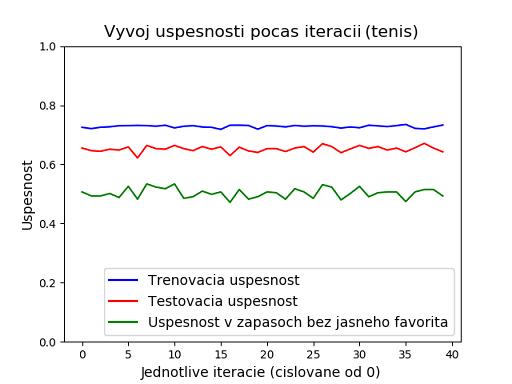
\includegraphics[width=\linewidth]{../img/ffnn_tenis_res.png} 
    \caption{Tenis} 
  \end{subfigure} 
  \begin{subfigure}[b]{0.48\linewidth}
    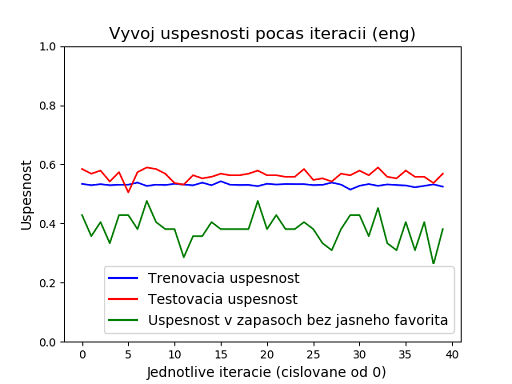
\includegraphics[width=\linewidth]{../img/ffnn_eng_res.png} 
    \caption{Futbal (anglická \textit{Premier league})} 
  \end{subfigure} 
  \begin{subfigure}[b]{0.48\linewidth}
    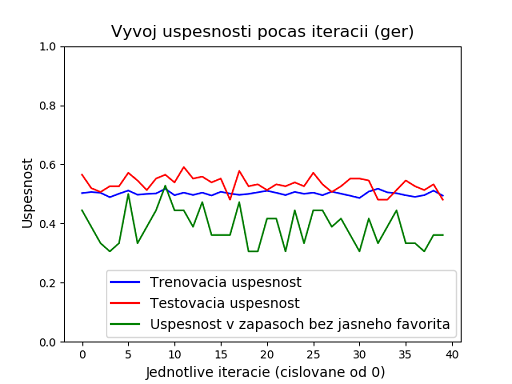
\includegraphics[width=\linewidth]{../img/ffnn_ger_res.png} 
    \caption{Futbal (nemecká \textit{Bundesliga})} 
  \end{subfigure}
  \hfill
  \begin{subfigure}[b]{0.48\linewidth}
    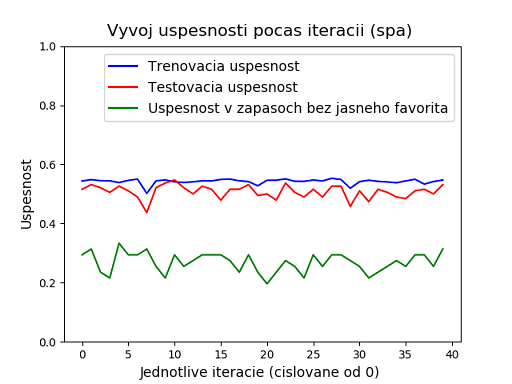
\includegraphics[width=\linewidth]{../img/ffnn_spa_res2.png} 
    \caption{Futbal (španielska \textit{La Liga})} 
  \end{subfigure}
  \caption{Výsledné trénovacie, testovacie úspešnosti a úspešnosti pri predikovaní zápasov bez jasného favorita} 
   \label{fig7} 
\end{figure}

Ak výsledky porovnáme s výsledkami získanými z kapitoly \ref{stavba}, kde sme pre\-di\-ko\-va\-li sezóny pred touto, tak vidíme, že nám sieť vydala iné výsledky.
V prípade tenisu sa to prejavilo mierne horšími hodnotami v sledovaných oblastiach, ale pri zápasoch bez jasného favorita došlo k výraznejšiemu poklesu.

V prípade futbalu pri španielskej lige ako jedinej došlo k poklesu testovacej úspešnosti a obrovský neúspech pre zápasy bez favorita, kde sieť zvolila správny výsledok len pri 26,86\,\% zápasov, čo je dokonca menej ako priemerná úspešnosť pri náhodnom zvolení výsledkov alebo tipovaním len domáceho tímu (obe sú viac ako 33\,\%).
V jednej sezóne sme dokonca dosiahli stratu skoro 25 jednotiek pri tipovaní 51 zápasov a úspešnosti pod 20\,\%, čo značí správne uhádnutých len 10 z 51 zápasov, ktoré v danej sezóne ligy nemali jasného favorita.

Na druhej strane nemecká aj anglická liga sa vyhodnocovali sieti o dosť lepšie ako pri trénovaní, v prípade nemeckej ligy bola testovacia úspešnosť vyššia o 2,5\,\% a v prípade anglickej dokonca o viac ako 5\,\%. Zaujímavosťou je, že úspešnosť v zápasoch bez favorita je na podobnej úrovni ako pri testovaní a celkový zisk sa pohybuje pri oboch ligách okolo 0.

Na obrázkoch \ref{fig7} a \ref{fig8} môžeme vidieť, ako sa vyvíjala trénovacia a testovacia úspešnosť a úspešnosť v zápasoch bez favorita a aký to malo dopad na celkový zisk. Konkrétne na obrázku \ref{fig7} a jeho častiach môžeme vidieť, že jednotlivé úspešnosti boli celkom konzistentné a zatiaľ čo celkové zisky zo zápasov bez favorita sa pohybovali chaotickejšie.


\begin{figure}[h!]
  \begin{subfigure}[b]{0.48\textwidth}
    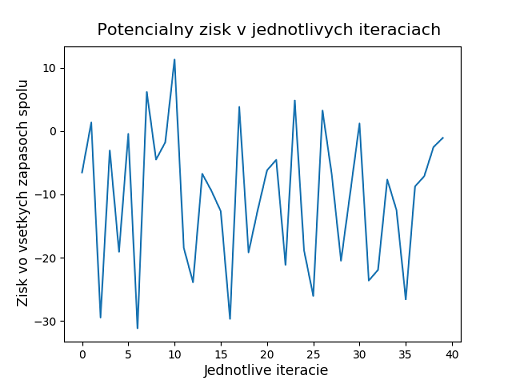
\includegraphics[width=\textwidth]{../img/ffnn_tenis_prof.png} 
    \caption{Tenis} 
  \end{subfigure} 
  \begin{subfigure}[b]{0.48\textwidth}
    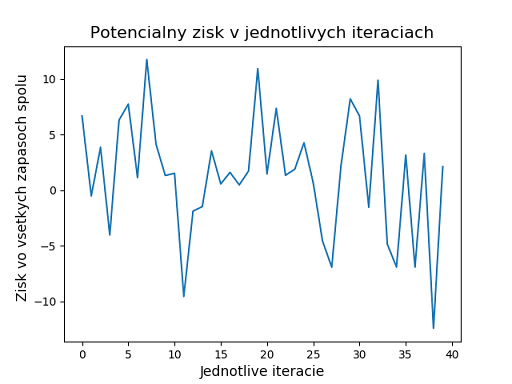
\includegraphics[width=\textwidth]{../img/ffnn_eng_prof.png} 
    \caption{Futbal (anglická \textit{Premier league})} 
  \end{subfigure} 
  \begin{subfigure}[b]{0.48\textwidth}
    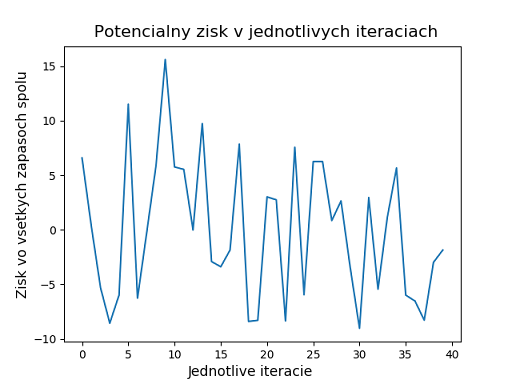
\includegraphics[width=\textwidth]{../img/ffnn_ger_prof.png} 
    \caption{Futbal (nemecká \textit{Bundesliga})} 
  \end{subfigure}
  \hfill
  \begin{subfigure}[b]{0.48\textwidth}
    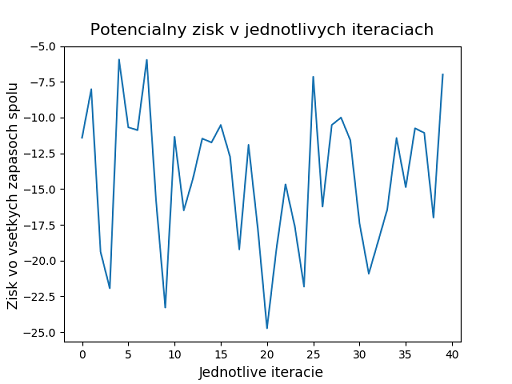
\includegraphics[width=\textwidth]{../img/ffnn_spa_prof.png} 
    \caption{Futbal (španielska \textit{La Liga})} 
  \end{subfigure}
  \caption{Výsledný zisk pri predikovaní zápasov bez jasného favorita (každý šport aj liga mali rôzny počet takýchto zápasov, tento obrázok ukazuje celkový zisk)} 
   \label{fig8} 
\end{figure}

Na obrázku \ref{fig9} môžeme vidieť testovacie úspešnosti pri pre\-dikovaní dvoch sezón, tmavšou farbou sú výsledky z tejto kapitoly, svetlejšou výsledky z kapitoly \ref{stavba}, teda výsledky z testovania a optimalizovania siete.
\begin{figure}[h!]
    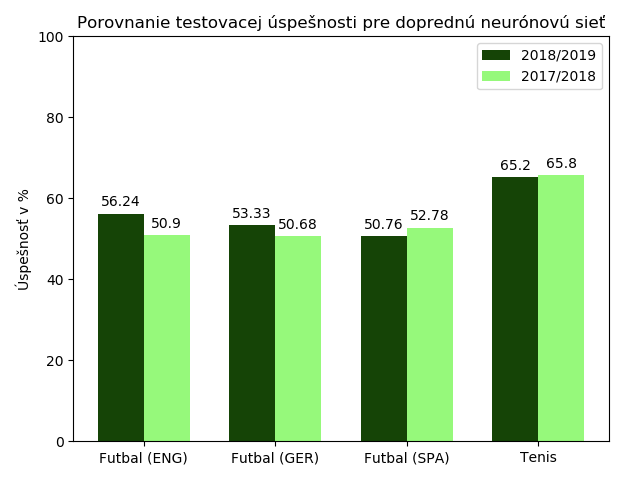
\includegraphics[width=\textwidth]{../img/ffnn_bars.png} 
    \caption{Porovnanie testovacej úspešnosti predikovaní poslednej a predposlednej sezóny. Úspešnosti z predposlednej sezóny (svetlá farba) prebehli pokusom o optimalizáciu a dané dáta aj model použitý pri predikovaní poslednej sezóny (tmavá farba)}
    \label{fig9} 
\end{figure}

\section{Rekurentná neurónová sieť}

Výsledky vyhodnocovania môžeme nájsť v tabuľke \ref{res_rnn}.

\begin{table}[h!]
\begin{center}
\begin{tabular}{ c|c|c|c|c|c| } 
 
 Šport (liga) & Tr \% &  Te \% & CG \% & CGP & CGP/M \\ 
 \hline 
 Futbal (ENG) & 52,44 & 56 & 37 & $-0,12$ & $-0,0029$\\ 
 Futbal (GER) & 49,88 & 50,54 & 38,68 & $-0,1$ & $-0,0028$ \\ 
 Futbal (SPA) & 53,98 & 51,51 & 28,87 & $-12,44$ & $-0,2439$\\
 Tenis & 73,07 & 65,67 & 48,14 & $-22,34$ & $-0,1064$ \\ 
 \hline
\end{tabular}
\caption{Priemerné výsledky vyhodnocovania cez 40 iterácií. Skratka Tr \% znamená trénovaciu úspešnosť, Te \% testovaciu úspešnosť. CG značí úspešnosť pri tipovaní zápasov bez favorita, CGP zisk pri uzatváraní stávok na tieto zápasy a CGP/M značí priemerný takýto zisk na zápas bez jasného favorita.}
\label{res_rnn}
\end{center}
\end{table}

\begin{figure}[h!] 
  \begin{subfigure}[b]{0.48\linewidth}
    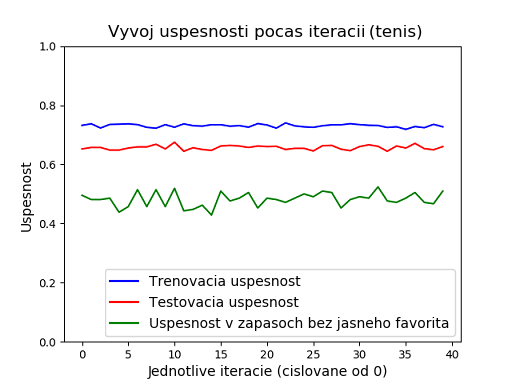
\includegraphics[width=\linewidth]{../img/rnn_tenis_res.png} 
    \caption{Tenis} 
  \end{subfigure} 
  \begin{subfigure}[b]{0.48\linewidth}
    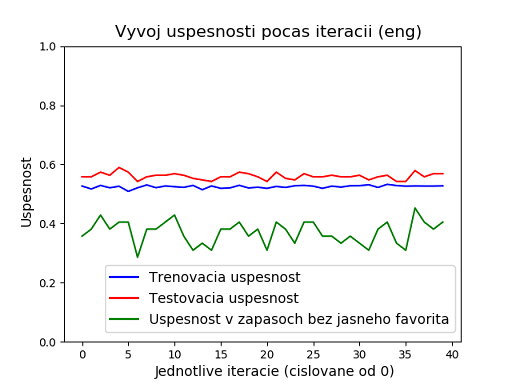
\includegraphics[width=\linewidth]{../img/rnn_eng_res.png} 
    \caption{Futbal (anglická \textit{Premier league})} 
  \end{subfigure} 
  \begin{subfigure}[b]{0.48\linewidth}
    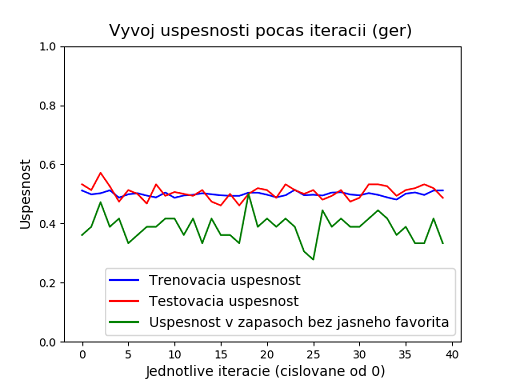
\includegraphics[width=\linewidth]{../img/rnn_ger_res.png} 
    \caption{Futbal (nemecká \textit{Bundesliga})} 
  \end{subfigure}
  \hfill
  \begin{subfigure}[b]{0.48\linewidth}
    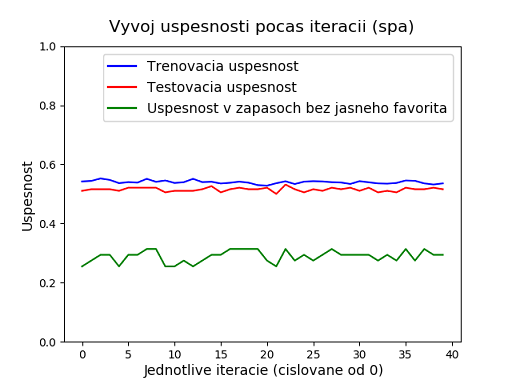
\includegraphics[width=\linewidth]{../img/rnn_spa_res3.png} 
    \caption{Futbal (španielska \textit{La Liga})} 
  \end{subfigure}
  \caption{Výsledné trénovacie, testovacie úspešnosti a úspešnosti pri predikovaní zápasov bez jasného favorita}
   \label{fig10} 
\end{figure}
Ak tieto výsledky porovnáme s výsledkami získanými pri rovnakej architektúre siete, ale pri vynechaní predposlednej sezóny z trénovacích dát a pre\-dikovaní tejto sezóny (sekcia \ref{rnn:train}), tak sa dozvieme, že nie sú až tak odlišné, s výnimkou anglickej futbalovej \textit{Premier league}, kde nastalo zlepšenie z 51,95\,\% na 56\,\%.
Toto zlepšenie ale nastalo na úkor úspešnosti v zápasoch bez jasného favorita, kde pri trénovaní sa dosiahla úspešnosť 39,2\,\% a celkový zisk 2,78 jednotky.

Najvýraznejší pokles oproti trénovaniu nastal v prípade španielskej \textit{La Ligy}, kde pri optimalizovaní siete bola testovacia úspešnosť 53,24\,\%, pri dátach z poslednej ukončenej sezóny dosiahla v priemere sieť úspešnosť 51,51\,\% a pri celkovom zisku pri hypotetickom uzatváraní stávok na zápasy bez favorita dopadla najhoršie z futbalových líg.
Horšie dopadol tenis, ten ale mal väčší počet zápasov bez jasného favorita.
Opäť treba dodať, že úspešnosť španielskej ligy v zápasoch bez favorita bola nižšia ako priemerná náhodná úspešnosť.

V prípade nemeckej \textit{Bundesligy} dopadla pre\-dikcia poslednej sezóny o niečo horšie ako v prípade tej predposlednej, všetky výsledky sú porovnateľné.

Pre tenis dopadla testovacia aj trénovacia úspešnosť mierne horšie, veľký pokles bol v úspešnosti pre\-dikcie zápasov bez favorita, kde prišiel pokles z 52\,\% na 48,14\,\% a to sa prejavilo aj na celkovom zisku v zápasoch bez favorita.

Na obrázkoch \ref{fig10} a \ref{fig11} môžeme vidieť, ako sa vyvíjala trénovacia a testovacia úspešnosť a úspešnosť v zápasoch bez favorita a aký to malo dopad na celkový zisk. Konkrétne na obrázku \ref{fig10} a jeho podobrázkoch môžeme vidieť, že jednotlivé úspešnosti boli celkom konzistentné (s výnimkou úspešnosti v zápasoch bez favorita, kde sa to mierne kolísalo), zatiaľ čo celkové zisky zo zápasov bez favorita (obrázok \ref{fig11}) sa pohybovali chaotickejšie.


\begin{figure}[h!]
  \begin{subfigure}[b]{0.48\textwidth}
    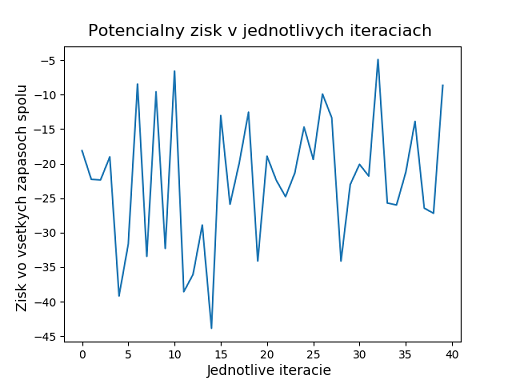
\includegraphics[width=\textwidth]{../img/rnn_tenis_prof.png} 
    \caption{Tenis} 
  \end{subfigure} 
  \begin{subfigure}[b]{0.48\textwidth}
    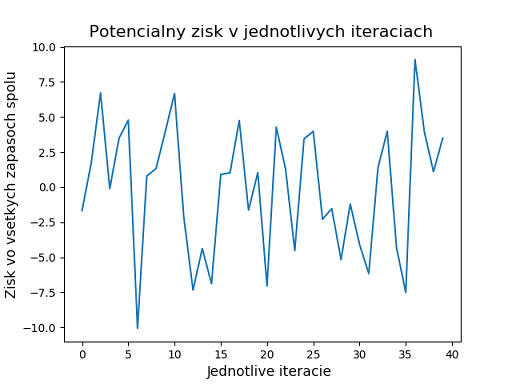
\includegraphics[width=\textwidth]{../img/rnn_eng_prof.png} 
    \caption{Futbal (anglická \textit{Premier league})} 
  \end{subfigure} 
  \begin{subfigure}[b]{0.48\textwidth}
    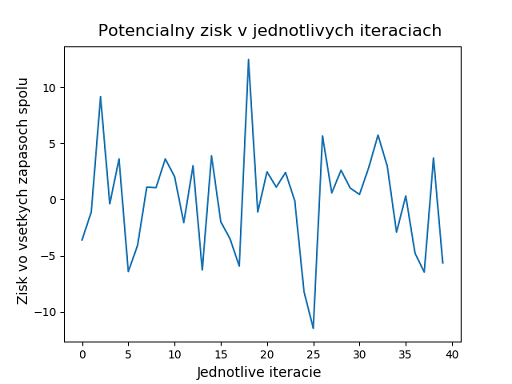
\includegraphics[width=\textwidth]{../img/rnn_ger_prof.png} 
    \caption{Futbal (nemecká \textit{Bundesliga})} 
  \end{subfigure}
  \hfill
  \begin{subfigure}[b]{0.48\textwidth}
    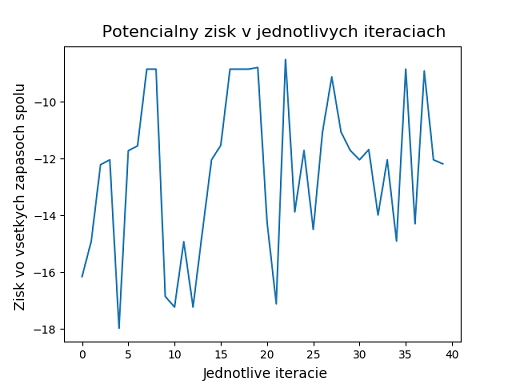
\includegraphics[width=\textwidth]{../img/rnn_spa_prof.png} 
    \caption{Futbal (španielska \textit{La Liga})} 
  \end{subfigure}
  \caption{Výsledný zisk pri predikovaní zápasov bez jasného favorita (každý šport aj liga mali rôzny počet takýchto zápasov, tento obrázok ukazuje celkový zisk)}
   \label{fig11}  
\end{figure}

Na obrázku \ref{fig12} môžeme vidieť testovacie úspešnosti pri pre\-dikovaní dvoch sezón, tmavšou farbou sú výsledky z tejto kapitoly, svetlejšou výsledky z kapitoly \ref{stavba}, teda výsledky z testovania a optimalizovania siete.

\begin{figure}[h!]
    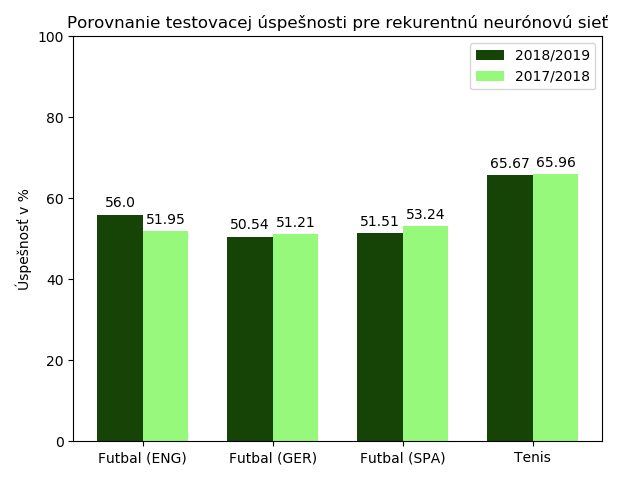
\includegraphics[width=\textwidth]{../img/rnn_bars.png} 
    \caption{Porovnanie testovacej úspešnosti predikovaní poslednej a predposlednej sezóny. Úspešnosti z predposlednej sezóny (svetlá farba) prebehli pokusom o optimalizáciu a dané dáta aj model použitý pri predikovaní poslednej sezóny (tmavá farba)}
    \label{fig12} 
\end{figure}

\section{Porovnanie}
Výsledky dosiahnuté v tejto kapitole boli odlišné, ako výsledky dosiahnuté v kapitole \ref{stavba}.
Videli sme, o koľko sa tieto výsledky líšili.
Môže to značiť mnohé veci, najskôr to ale značí fakt, že každá sezóna má vlastnú predvídateľnosť a aj keď dokážeme sieť naučiť predpovedať jednu sezónu, neznamená to, že rovnaká architektúra bude úspešná aj pri inej sezóne, nie to ešte inej lige alebo športe. V našom prípade sa nám podarilo poraziť stávkové kancelárie len v prípade doprednej neurónovej siete na pre\-dikciu anglickej \textit{Premier League}, aj to len o 1,35 jednotky, čo v preklade znamená, že ak by sme celú sezónu uzatvárali stávky na zápasy bez favorita tak, ako by nám to predpovedala naša sieť a na každý zápas by sme vsadili rovnakú čiastku, tak by sme na konci ostali v zisku, ktorý by sa rovnal 1,35-násobku jedného vkladu.

Na vychýlenie úspešnosti siete vo futbalovej lige zo sezóny na sezónu stačí, ak jeden z dvoch najlepších hráčov sveta prestúpi medzi sezónou do inej ligy a jeho tím nebude bez neho dosahovať rovnaké výsledky \citep{ronaldo}. 
Zdá sa, že obe siete sa v tomto prípade, minimálne zo začiatku sezóny opierali o údaje o dlhodobej sile tímov (príznaky 41 a 42 v Prílohe \ref{in:foot}), čo mohlo viesť k miernemu poklesu úspešnosti tak, ako sme videli.
V anglickej lige sme zaznamenali vzostup aj v trénovacej a aj v testovacej úspešnosti, čo potvrdzuje teóriu o rozličnej predvídateľnosti rozličných sezón.

Zo získaných údajov sme zistili mimo iného aj to, ako sa zmenila predvídateľnosť jednotlivých športových výsledkov z roka na rok (sezóny na sezónu).
Môžeme povedať, že pre\-dikovaná sezóna anglickej \textit{Premier League} bola ľahšie predvídateľná ako tá minulá. Na druhej strane horšie sa obom typom sietí pre\-dikovala španielska \textit{La Liga}. Tieto poznatky môžeme zformulovať do pár hypotéz o rozdiele medzi doprednou a rekurentnou neurónovou sieťou.

Ak je sezóna výrazne horšie predvídateľná ako sezóna, z ktorej sú data, tak oba modely prezentované v tejto práci vykazujú horšie výsledky. Rekurentná neurónová sieť vykazuje mierne lepšie výsledky, LSTM neuróny aj s ich implementáciou krátkodobej pamäte pomáhajú v tomto ohľade sieti.

Naopak, ak je sezóna lepšie predvídateľná ako predchádzajúce, tak obe modely dosahujú vyššej testovacej ako trénovacej úspešnosti. Dopredná neurónová sieť dosahuje o niečo lepšie výsledky, čo môže znamenať, že pamäť rekurentnej neurónovej siete núti túto sieť rozmýšľať konzervatívnejšie.

Celkovo ale sú výsledky veľmi podobné na to, aby sa dali s určitosťou vysloviť nejaké tvrdenia o prezentovaných typoch neurónových sietí.

Na obrázku \ref{fig20} môžeme vidieť rozdiel v úspešnosti medzi najlepšími modelmi doprednej a rekurentnej neurónovej siete podľa kapitoly \ref{stavba} pri pre\-dikcii vyhodnocovanej sezóny (sezóny 2018/2019).

\begin{figure}[t]
    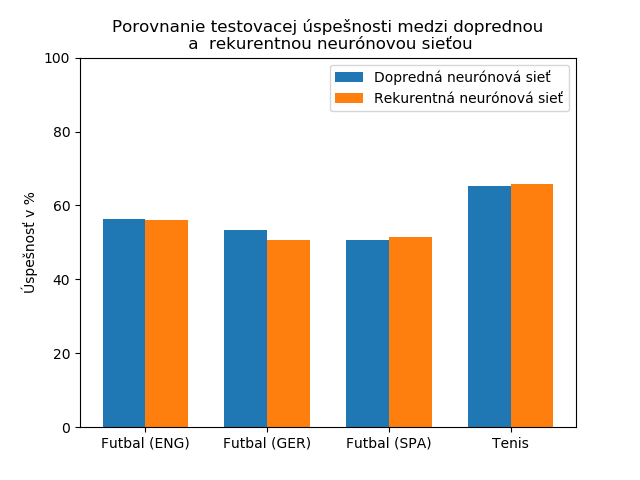
\includegraphics[width=\textwidth]{../img/bars.png} 
    \caption{Porovnanie testovacej úspešnosti modelov doprednej (modrá farba) a rekurentnej (oranžová) neurónovej siete pri predikcii výsledkov jednotlivých líg}
    \label{fig20} 
\end{figure}

\chapter*{Záver}
\addcontentsline{toc}{chapter}{Záver}

Jedným z dôvodov, prečo ľudia sledujú šport je ten, že šport je nepredvídateľný. Na druhej strane, ľudstvo sa učí od nepamäti získavať kontrolu nad nepredvídateľným a ak sa to nepodarí, tak aspoň to s nejakou určitosťou predvídať (napríklad zatmenie slnka). Vedieť predvídať športové výsledky by nám zaručilo nielen slávu a pozornosť médií, ale mohlo by nám to pred týmto všetkým zaručiť aj bohatstvo, pretože stávkové kancelárie dávajú možnosť zarobiť na správnom tipovaní (v našom prípade predpovedaní) výsledkov.

Jedným z relatívne nových spôsobov, ktorý sa začína používať na predpovedanie športových výsledkov je strojové učenie. Jedným z najznámejších a momentálne aj naobľúbenejších typov strojového učenia sú neurónové siete. V tejto práci sme sa zamerali na dva druhy neurónových sietí, a to dopredné a rekurentné neurónové siete a ich úspešnosť pri predikcii výsledkov v troch futbalových ligách a na najvyšších tenisových turnajoch medzi najlepšími hráčmi.

Používali sme len dáta, ktoré vieme vyčítať z výsledkov (v prípade tenisu aj z koncoročných rebríčkov), ale nepodarilo sa nám ani priblížiť výsledkom iných autorov publikujúcich v tejto oblasti, ktorý používali aj fakticky nepodložené abstraktné dáta od expertov v oblasti. V prípade futbalu sme dosiahli úspešnosť od 50,54 -- 56,24 \,\%. V prípade tenisu sme dosiahli úspešnosť okolo 65,5\,\%.

Jednou z odlišností tejto práce od ostatných v oblasti bolo zameranie sa aj na zápasy bez jasného favorita stávkových kancelárií. Aj napriek tomu, že to bol celkom nový prístup, nepodarilo sa nám dosiahnúť požadované výsledky, ktoré by mohli podnietiť väčší výskum týmto smerom. To ale neznamená, že sa lepšie výsledky dosiahnuť nedajú. Znamená to iba, že sa zo získaných dát ukázaným spôsobom nebude dať vytvoriť neurónová ani rekurentná neurónová sieť, ktorá by dosahovala stabilné výsledky a dokázala by pravidelne a dlhodobo poraziť stávkové kancelárie a vykázať teda nejaký zisk.

%%% Seznam použité literatury
%%% Seznam použité literatury (bibliografie)
%%%
%%% Pro vytváření bibliografie používáme bibTeX. Ten zpracovává
%%% citace v textu (např. makro \cite{...}) a vyhledává k nim literaturu
%%% v souboru literatura.bib.
%%%
%%% Příkaz \bibliographystyle určuje, jakým stylem budou citovány odkazy
%%% v textu. V závorce je název zvoleného souboru .bst. Styly plainnat
%%% a unsrt jsou standardní součástí latexových distribucí. Styl czplainnat
%%% je dodáván s touto šablonou a bibTeX ho hledá v aktuálním adresáři.

 \bibliographystyle{czplainnat}    %% Autor (rok) s českými spojkami
% \bibliographystyle{plainnat}    %% Autor (rok) s anglickými spojkami
% \bibliographystyle{unsrt}       %% [číslo]
% \bibliographystyle{abbrv}

%\renewcommand{\bibname}{Seznam použité literatury}
\renewcommand{\bibname}{Zoznam použitej literatúry}

%%% Vytvoření seznamu literatury. Pozor, pokud jste necitovali ani jednu
%%% položku, seznam se automaticky vynechá.
\sloppy
\bibliography{literatura}

%%% Kdybyste chtěli bibliografii vytvářet ručně (bez bibTeXu), lze to udělat
%%% následovně. V takovém případě se řiďte normou ISO 690 a zvyklostmi v oboru.

% \begin{thebibliography}{99}
%
% \bibitem{lamport94}
%   {\sc Lamport,} Leslie.
%   \emph{\LaTeX: A Document Preparation System}.
%   2. vydání.
%   Massachusetts: Addison Wesley, 1994.
%   ISBN 0-201-52983-1.
%
% \end{thebibliography}


%%% Obrázky v bakalářské práci
%%% (pokud jich je malé množství, obvykle není třeba seznam uvádět)
% \listoffigures

%%% Tabulky v bakalářské práci (opět nemusí být nutné uvádět)
%%% U matematických prací může být lepší přemístit seznam tabulek na začátek práce.
% \listoftables

%%% Použité zkratky v bakalářské práci (opět nemusí být nutné uvádět)
%%% U matematických prací může být lepší přemístit seznam zkratek na začátek práce.
% \chapwithtoc{Seznam použitých zkratek}

%%% Přílohy k bakalářské práci, existují-li. Každá příloha musí být alespoň jednou
%%% odkazována z vlastního textu práce. Přílohy se číslují.
%%%
%%% Do tištěné verze se spíše hodí přílohy, které lze číst a prohlížet (dodatečné
%%% tabulky a grafy, různé textové doplňky, ukázky výstupů z počítačových programů,
%%% apod.). Do elektronické verze se hodí přílohy, které budou spíše používány
%%% v elektronické podobě než čteny (zdrojové kódy programů, datové soubory,
%%% interaktivní grafy apod.). Elektronické přílohy se nahrávají do SISu a lze
%%% je také do práce vložit na CD/DVD. Povolené formáty souborů specifikuje
%%% opatření rektora č. 72/2017.
\appendix
\chapter{Prílohy}

\section{Vstup neurónovej siete pre futbal} \label{in:foot}
Výstupný súbor z transformačnej časti predikcie pre futbal je tabuľka formátu \textit{csv}. Riadky predstavujú jednotlivé predikované zápasy a stĺpce sú nasledovné:
\begin{enumerate}
 \item htW - home team wins - doterajší počet výher domáceho tímu v práve evaluovanej sezóne,
 \item htD - home team draws - doterajší počet remíz domáceho tímu v práve evaluovanej sezóne,
 \item htL - home team loses - doterajší počet prehier domáceho tímu v práve evaluovanej sezóne,
 \item htGFpG - home team goals for per game - doterajší priemerný počet strelených gólov na zápas domáceho tímu v práve evaluovanej sezóne,
 \item htGApG - home team goals against per game - doterajší priemerný počet inkasovaných gólov na zápas domáceho tímu v práve evaluovanej sezóne,
 \item atW - away team wins - doterajší počet výher hosťujúceho tímu v práve evaluovanej sezóne,
 \item atD - away team draws - doterajší počet remíz hosťujúceho tímu v práve evaluovanej sezóne,
 \item atL - away team loses - doterajší počet prehier hosťujúceho tímu v práve evaluovanej sezóne,
 \item atGFpG - away team goals for per game - doterajší priemerný počet strelených gólov na zápas hosťujúceho tímu v práve evaluovanej sezóne,
 \item atGApG - away team goals against per game - doterajší priemerný počet inkasovaných gólov na zápas hosťujúceho tímu v práve evaluovanej sezóne,
 \item htHW - home team home wins - doterajší počet výher domáceho tímu na domácom ihrisku v práve evaluovanej sezóne,
 \item htHD - home team home draws - doterajší počet remíz domáceho tímu na domácom ihrisku v práve evaluovanej sezóne,
 \item htHL - home team home loses - doterajší počet prehier domáceho tímu na domácom ihrisku v práve evaluovanej sezóne,
 \item htHGFpG - home team home goals for per game - doterajší priemerný počet strelených gólov na zápas domáceho tímu na domácom ihrisku v práve evaluovanej sezóne,
 \item htHGApG - home team home goals against per game - doterajší priemerný počet inkasovaných gólov na zápas domáceho tímu na domácom ihrisku v práve evaluovanej sezóne,
 \item atAW - away team away wins - doterajší počet výher hosťujúceho tímu v role hostí v práve evaluovanej sezóne,
 \item atAD - away team away draws - doterajší počet remíz hosťujúceho tímu v role hostí v práve evaluovanej sezóne,	 
 \item atAL - away team away loses - doterajší počet prehier hosťujúceho tímu v role hostí v práve evaluovanej sezóne,
 \item atAGFpG - away team away goals for per game - doterajší priemerný počet strelených gólov na zápas hosťujúceho tímu v role hostí v práve evaluovanej sezóne,
 \item atAGApG - away team away goals against per game - doterajší priemerný počet inkasovaných gólov na zápas hosťujúceho tímu v role hostí v práve evaluovanej sezóne,
 \item hFW - home form wins - počet výher domáceho tímu v posledných 5 zápasoch,
 \item hFD - home form draws - počet remíz domáceho tímu v posledných 5 zápasoch,
 \item hFL - home form loses - počet prehier domáceho tímu v posledných 5 zápasoch,
 \item hFGF - home form goals for - priemerný počet strelených gólov domáceho tímu v posledných 5 zápasoch,
 \item hFGA - home form goals against - priemerný počet inkasovaných gólov domáceho tímu v posledných 5 zápasoch,
 \item aFW - away form wins - počet výher hosťujúceho tímu v posledných 5 zápasoch, 
 \item aFD - away form draws - počet remíz hosťujúceho tímu v posledných 5 zápasoch,
 \item aFL - away form loses - počet prehier hosťujúceho tímu v posledných 5 zápasoch,
 \item aFGF - away form goals for - priemerný počet strelených gólov hosťujúceho tímu v posledných 5 zápasoch,
 \item aFGA - away form goals against - priemerný počet inkasovaných gólov hosťujúceho tímu v posledných 5 zápasoch,
 \item MW - mutual wins - počet výhier domáceho tímu v posledných 5 vzájomných zápasoch proti hosťujúcemu tímu (alebo všetkých vzájomných zápasoch od prvej sezóny v dátasete),
 \item MD - mutual draws - počet remíz domáceho tímu v posledných 5 vzájomných zápasoch proti hosťujúcemu tímu,
 \item ML - mutual loses - počet prehier domáceho tímu v posledných 5 vzájomných zápasoch proti hosťujúcemu tímu,
 \item MGF - mutual goals for - priemerný počet strelených gólov domáceho tímu v posledných 5 vzájomných zápasoch proti hosťujúcemu tímu,
 \item MGA - mutual goals against - priemerný počet inkasovaných gólov domáceho tímu v posledných 5 vzájomných zápasoch proti hosťujúcemu tímu,
 \item MhW - mutual home wins - počet výhier domáceho tímu v posledných 5 vzájomných zápasoch proti hosťujúcemu tímu hraných na domácom ihrisku,
 \item MhD - mutual home draws - počet remíz domáceho tímu v posledných 5 vzájomných zápasoch proti hosťujúcemu tímu hraných na domácom ihrisku,
 \item MhL - mutual home loses - počet prehier domáceho tímu v posledných 5 vzájomných zápasoch proti hosťujúcemu tímu hraných na domácom ihrisku,
 \item MhGF - mutual home goals for - priemerný počet strelených gólov domáceho tímu v posledných 5 vzájomných zápasoch proti hosťujúcemu tímu hraných na domácom ihrisku,
 \item MhGA - mutual home goals against - priemerný počet inkasovaných gólov domáceho tímu v posledných 5 vzájomných zápasoch proti hosťujúcemu tímu hraných na domácom ihrisku,
 \item htLTS - home team long-time strength - dlhodobá sila domáceho mužstva (počítaná ako priemerný počet získaných bodov vo všetkých doterajších sezónach od prvej sezóny v dátasete),
 \item atLTS - away team long-time strength - dlhodobá sila hosťujúceho mužstva,
 \label{dFS}
 \item dFS - difference form score - rozdiel v skóre formy medzi domácim a hosťujúcim tímom,
 \item dFCS - difference form current score - rozdiel v momentálnom skóre formy medzi domácim a hosťujúcim tímom,
 \item H - home - hodnota určujúca konečný výsledok zápasu; 1, ak skončil víťazstvom domáceho tímu, 0 inak,
 \item D - draw - hodnota určujúca konečný výsledok zápasu; 1, ak skončil remízou, 0 inak, 
 \item A - away - hodnota určujúca konečný výsledok zápasu; 1, ak skončil prehrou domáceho tímu, 0 inak.
\end{enumerate}

Skóre formy oboch tímov je vypočítané ako súčet cez posledných 5 zápasov počet bodov súpera tímu v momente ukončenia zápasu vynásobený počtom bodov získaných z daného zápasu.
To by malo ukázať silu výsledku a dať dôraz na neskôr odohrané zápasy.
Momentálne skóre formy funguje podobne s výnimkou toho, že je prepočítavané pred evaluovaným zápasom a nie v momente ukončenia zápasu, čo by malo viac ukázať silu výsledku s odstupom času.

Súbory používané na testovanie a vyhodnocovanie siete obsahujú ešte 3 stĺpce pre každý riadok, v poradí kurz na výhru domáceho mužstva, kurz na remízu a kurz na výhru hosťujúceho mužstva.


\section{Vstup neurónovej siete pre tenis} \label{in:ten}
Výstupný súbor z transformačnej časti predikcie pre tenis je tabuľka vo formáte \textit{csv}. Riadky predstavujú jednotlivé predikované zápasy a stĺpce sú nasledovné:

\begin{enumerate}
 \item 1W - player 1 wins - počet výher hráča 1 v práve vyhodnocovanej sezóne,
 \item 1L - player 1 loses - počet prehier hráča 1 v práve vyhodnocovanej sezóne,
 \item 1GDpS - player 1 game difference per set - priemerný rozdiel v počte vyhraných a prehraných hier za set hráča 1 v práve vyhodnocovanej sezóne,
 \item 2W - player 2 wins - počet výher hráča 2 v práve vyhodnocovanej sezóne,
 \item 2L - player 2 loses - počet prehier hráča 2 v práve vyhodnocovanej sezóne,
 \item 2GDpS - player 2 game difference per set - priemerný rozdiel v počte vyhraných a prehraných hier za set hráča 2 v práve vyhodnocovanej sezóne,
 \item 1FW - player 1 form wins - počet výher hráča 1 v jeho posledných 10 zápasoch,
 \item 1FL - player 1 form loses - počet prehier hráča 1 v jeho posledných 10 zápasoch,
 \item 1FGDpS - player 1 form game difference per set - priemerný rozdiel v počte vyhraných a prehraných hier za set hráča 1 v jeho posledných 10 zápasoch,
 \item 2FW - player 2 form wins - počet výher hráča 2 v jeho posledných 10 zápasoch,
 \item 2FL - player 2 form loses - počet prehier hráča 2 v jeho posledných 10 zápasoch,
 \item 2FGDpS - player 2 form game difference per set - priemerný rozdiel v počte vyhraných a prehraných hier za set hráča 2 v jeho posledných 10 zápasoch,
 \item 1SW - player 1 surface wins - počet výher hráča 1 na danom povrchu v práve vyhodnocovanej sezóne,
 \item 1SL - player 1 surface loses - počet prehier hráča 1 na danom povrchu v práve vyhodnocovanej sezóne,
 \item 1SGDpS - player 1 surface game difference per set - priemerný rozdiel v počte vyhraných a prehraných hier za set hráča 1 na danom povrchu v práve vyhodnocovanej sezóne,
 \item 2SW - player 2 surface wins - počet výher hráča 2 na danom povrchu v práve vyhodnocovanej sezóne,
 \item 2SL - player 2 surface loses - počet prehier hráča 2 na danom povrchu v práve vyhodnocovanej sezóne,
 \item 2SGDpS - player 2 surface game difference per set - priemerný rozdiel v počte vyhraných a prehraných hier za set hráča 2 na danom povrchu v práve vyhodnocovanej sezóne,
 \item 1SFW - player 1 surface form wins - počet výher hráča 1 v jeho posledných 10 zápasoch odohraných na danom povrchu,
 \item 1SFL - player 1 surface form loses - počet prehier hráča 1 v jeho posledných 10 zápasoch odohraných na danom povrchu,
 \item 1SFGDpS - player 1 surface form game difference per set - priemerný rozdiel v počte vyhraných a prehraných hier za set hráča 1 na danom povrchu v jeho posledných 10 zápasoch,
 \item 2SFW - player 2 surface form wins - počet výher hráča 2 v jeho posledných 10 zápasoch odohraných na danom povrchu,
 \item 2SFL - player 2 surface form loses - počet prehier hráča 2 v jeho posledných 10 zápasoch odohraných na danom povrchu,
 \item 2SFGDpS - player 2 surface form game difference per set - priemerný rozdiel v počte vyhraných a prehraných hier za set hráča 1 na danom povrchu v jeho posledných 10 zápasoch,
 \item 1MW - player 1 mutual wins - počet výher hráča 1 vo vzájomných zápasoch*,
 \item 1ML - player 1 mutual loses - počet prehier hráča 1 vo vzájomných zápasoch*,
 \item 1MGDpS - player 1 mutual game difference per set - priemerný rozdiel v počte vyhraných a prehraných hier za set hráča 1 vo vzájomných zápasoch*,
 \item 1MSW - player 1 mutual surface wins - počet výher hráča 1 vo vzájomných zápasoch* odohraných na danom povrchu, 
 \item 1MSL - player 1 mutual surface loses - počet prehier hráča 1 vo vzájomných zápasoch* odohraných na danom povrchu,
 \item 1MSGDpS - player 1 mutual surface game difference per set - priemerný rozdiel v počte vyhraných a prehraných hier za set hráča 1 vo vzájomných zápasoch* odohraných na danom povrchu,
 \item 1R - player 1 rank - umiestnenie hráča 1 v poslednom koncoročnom rebríčku ATP
 \item 2R - player 2 rank - umiestnenie hráča 2 v poslednom koncoročnom rebríčku ATP
 \item H - hard - kategorická hodnota určujúca povrch, na ktorom sa odohral zápas; 1, ak sa hral na tvrdom povrchu, 0 inak
 \item C  - clay - kategorická hodnota určujúca povrch, na ktorom sa odohral zápas; 1, ak sa hral na antuke, 0 inak
 \item G - grass - kategorická hodnota určujúca povrch, na ktorom sa odohral zápas; 1, ak sa hral na trávnatom povrchu, 0 inak
 \item dSc - difference in score - rozdiel v skóre oboch hráčov**,
 \item dSSc - difference in surface score - rozdiel v skóre oboch hráčov na danom povrchu**,
 \item 1? - did player 1 win - hodnota určujúca víťaza; 1, ak vyhral hráč 1, 0 inak
 \item 2? - did player 2 win - hodnota určujúca víťaza; 1, ak vyhral hráč 2, 0 inak
\end{enumerate}
* - vzájomné zápasy sú prepočítavané len pre sezóny, odkiaľ sú dáta; tie sú od sezóny 2003, najstaršie trénovacie dáta obsahujú sezónu 2012, takže to teoreticky môže ovplyvniť len zápasy medzi hráčmi, ktorí hrajú profesionálne viac ako 9 rokov a aspoň jeden z nich sa už vtedy umiestnil v Top 100 rebríčka ATP a v práve evaluovanej sezóne sa tam umiestnili obaja; to sa nestávalo často, efekt to malo na minimum vyhodnocovaní a teória hovorí, že posledné vzájomné zápasy sú aj ak dôležitejšie, takže teoreticky nevadí, že je konečná sezóna, ak je ďaleko od práve vyhodnocovanej.\\
** - skóre je pokus ohodnotiť silu víťazstva, berie do úvahy formu, teda posledných 10 zápasov a počíta sa ako $(150 - rank)\cdot point$, kde rank je poradie súpera v poslednom koncoročnom rebríčku ATP a point je nastavené na 1, ak hráč vyhral, a na 0, ak prehral. 
Ak súper nebol v Top 100 rebríčka ATP na konci predchádzajúceho roka, tak za jeho rank je dosadené číslo 130.
To je len preto, lebo teoreticky má dané víťazstvo hodnotu, musí byť teda nejak ohodnotené lepšie ako ľubovoľná prehra, ktorá je ohodnotená hodnotou 0.

Súbory používané na testovanie a vyhodnocovanie siete obsahujú ešte 2 stĺpce pre každý riadok, v poradí kurz na výhru hráča 1 a kurz na výhru hráča 2.

\openright
\end{document}
